\documentclass[12pt, a4paper]{report}
\usepackage[english]{babel}
\usepackage{titlesec}

\titleformat{\chapter} % command
  [display] % shape
  {\bfseries\huge} % format
  {Chapter \thechapter} % label
  {0pt} % sep
  {} % before-code


\usepackage[T5]{fontenc}
\usepackage{mathptmx}[ptm]
\usepackage{a4wide, amssymb, epsfig, latexsym, array, hhline, fancyhdr}
\usepackage[normalem]{ulem}
%\usepackage{soul}
\usepackage{float}
\usepackage[makeroom]{cancel}
\usepackage{amsmath}
\usepackage{amsthm}
\usepackage{multicol, longtable, amscd}
\usepackage{diagbox}%Make diagonal lines in tables
\usepackage{booktabs}
\usepackage{alltt}
\usepackage[framemethod=tikz]{mdframed}% For highlighting paragraph backgrounds
\usepackage{indentfirst}
\usepackage{caption,subcaption}
\usepackage{svg}
\graphicspath{ {figures/} }
\usepackage{lastpage}
\usepackage[lined,boxed,commentsnumbered]{algorithm2e}
\usepackage{enumerate}
\usepackage{color}
\usepackage{graphicx}% Standard graphics package
\graphicspath{ {figures/} }
\usepackage{array}
\usepackage{tabularx, caption}
\usepackage{tabularray}
\usepackage{multirow}
\usepackage{multicol}
\usepackage{rotating}
\usepackage{graphics}
\usepackage{geometry}
\usepackage{setspace}
\usepackage{epsfig}
\usepackage{tikz}
\usepackage[numbers]{natbib}
\usepackage{subcaption}

\usepackage{dirtree}



\usetikzlibrary{arrows, snakes, backgrounds, calc}
\usepackage[unicode]{hyperref}
\hypersetup{urlcolor=blue,linkcolor=black,citecolor=black,colorlinks=true} 

\usepackage{xcolor}

\definecolor{codegreen}{rgb}{0,0.6,0}
\definecolor{codegray}{rgb}{0.5,0.5,0.5}
\definecolor{codepurple}{rgb}{0.58,0,0.82}
\definecolor{backcolour}{rgb}{0.95,0.95,0.92}

\usepackage{listings}
\lstdefinestyle{mystyle}{
    backgroundcolor=\color{backcolour},   
    commentstyle=\color{codegreen},
    keywordstyle=\color{magenta},
    numberstyle=\tiny\color{codegray},
    stringstyle=\color{codepurple},
    basicstyle=\ttfamily\footnotesize,
    breakatwhitespace=false,         
    breaklines=true,                 
    captionpos=b,                    
    keepspaces=true,                 
    numbers=left,                    
    numbersep=5pt,                  
    showspaces=false,                
    showstringspaces=false,
    showtabs=false,                  
    tabsize=2
}
\lstset{style=mystyle}



\def\thesislayout{	% A4: 210 × 297
	\geometry{
		a4paper,
		total={160mm,240mm},  % fix over page
		left=30mm,
		top=30mm,
	}
}
\thesislayout

%\usepackage{fancyhdr}
\setlength{\headheight}{40pt}
\pagestyle{fancy}
\fancyhead{} % clear all header fields
\fancyhead[L]{
 \begin{tabular}{rl}
    \begin{picture}(25,15)(0,0)
    \put(0,-8){
\includegraphics[width=10mm, height=10mm]{Images/hcmut.png}}
    %\put(0,-8){\epsfig{width=10mm,figure=hcmut.eps}}
   \end{picture}&
	%
\includegraphics[width=8mm, height=8mm]{hcmut.png} & %
	\begin{tabular}{l}
        \textbf{ Vietnam National University, Ho Chi Minh City} \\
        \textbf{ Faculty of Computer Science and Engineering }
	\end{tabular} 	
 \end{tabular}
}
\fancyhead[R]{
	\begin{tabular}{l}
		\tiny \bf \\
		\tiny \bf 
	\end{tabular}  }
\fancyfoot{} % clear all footer fields
\fancyfoot[L]{\scriptsize Capstone Project Report (CO4029) - Academic year 2023 - 2024}
\fancyfoot[R]{\scriptsize  Page {\thepage}/\pageref{LastPage}}
\renewcommand{\headrulewidth}{0.3pt}
\renewcommand{\footrulewidth}{0.3pt}

%%%%%%%%%%%%%%%%%%%%%%%%%%%%%%%%%%%%%%%%%%
% Tạo một môi trường mới cho các bảng đặc tả UC, giúp định dạng kiểu
\newenvironment{usecase_table}[1][Test]
{
\begin{table}[H]
% Left-Right Table padding
    \setlength{\tabcolsep}{6pt}
    \renewcommand{\arraystretch}{1.5}
    % \begin{tabularx}{\textwidth}{bs}
    \def\savedcaption{\caption{#1}}%
    \begin{tabular}{|>{\bfseries} p{0.2\linewidth}|p{0.7\linewidth}|}

}
{
    \end{tabular}
    \savedcaption
\end{table}
}

\newenvironment{usecase_enum}
{
    \begin{enumerate*}[itemjoin={\newline}]
}
{
    \end{enumerate*}
}

\makeatletter
\newenvironment{acknowledgments}{
	\small
	\begin{center}
	  {\bfseries Acknowledgments\vspace{-.5em}\vspace{\z@}}
	\end{center}
	\quotation
  }{}
\makeatother

% Declaration
\makeatletter
\newenvironment{declaration}{
	\small
	\begin{center}
	  {\bfseries Declaration\vspace{-.5em}\vspace{\z@}}
	\end{center}
	\quotation
  }{}
\makeatother

\makeatletter
\newenvironment{abstr}{
        \small
        \begin{center}
	{\bfseries Abstract \vspace{-.5em}\vspace{\z@}}
        \end{center}
        \quotation
    }{}
\makeatother

\makeatletter
\newenvironment{abstrsss}{
        \small
        \begin{center}
	{\bfseries Abstractss \vspace{-.5em}\vspace{\z@}}
        \end{center}
        \quotation
    }{}
\makeatother
%%%%%%%%%%%%%%%%%%%%%%%%%%%%%%%%%%%%%%%%%%%%%%5
\setcounter{secnumdepth}{4}
\setcounter{tocdepth}{3}
\makeatletter
\newcounter {subsubsubsection}[subsubsection]
\renewcommand\thesubsubsubsection{\thesubsubsection .\@alph\c@subsubsubsection}
\newcommand\subsubsubsection{\@startsection{subsubsubsection}{4}{\z@}%
                                     {-3.25ex\@plus -1ex \@minus -.2ex}%
                                     {1.5ex \@plus .2ex}%
                                     {\normalfont\normalsize\bfseries}}
\newcommand*\l@subsubsubsection{\@dottedtocline{3}{10.0em}{4.1em}}
\newcommand*{\subsubsubsectionmark}[1]{}
\makeatother



\everymath{\color{black}}%make in-line maths symbols blue to read/check easily

\sloppy
\captionsetup[figure]{labelfont={small,bf},textfont={small,it},belowskip=-1pt,aboveskip=-9pt}
%space removed between caption, figure, and text
\captionsetup[table]{labelfont={small,bf},textfont={small,it},belowskip=-1pt,aboveskip=7pt}
\setlength{\floatsep}{5pt plus 2pt minus 2pt}
\setlength{\textfloatsep}{5pt plus 2pt minus 2pt}
\setlength{\intextsep}{10pt plus 2pt minus 2pt}


% Declare a variable named Proc using \newcommand
\newcommand{\Proc}{Assoc. Prof. Dr. Lê Hồng Trang }

\newcommand{\Uni}{Ho Chi Minh University - Vietnam National Unversity, Ho Chi Minh City}

\renewcommand{\labelitemi}{\normalfont\bfseries\textendash}
\renewcommand{\labelitemii}{\textbullet}
\renewcommand*\baselinestretch{1.5}\selectfont

\thesislayout

\begin{document}

\begin{titlepage}
    
\begin{tikzpicture}[remember picture, overlay]
        \draw[line width = 4pt] ($(current page.north west) + (1.0in,-0.5in)$) rectangle ($(current page.south east) + (-0.4in,0.5in)$);
        \draw[line width=1.5pt]
        ($ (current page.north west) + (1.05in,-0.55in) $)
        rectangle
        ($ (current page.south east) + (-0.45in,0.55in) $);
    \end{tikzpicture}

    \begin{center}
        \large \textbf{VIETNAM NATIONAL UNIVERSITY, HO CHI MINH CITY} \\
        \large \textbf{HO CHI MINH UNIVERSITY OF TECHNOLOGY} \\
        \large \textbf{FACULTY OF COMPUTER SCIENCE AND ENGINEERING}
    \end{center}

    \begin{figure}[h!]
        \begin{center}
            
\includegraphics[width=5cm]{Images/hcmut.png}
        \end{center}
    \end{figure}

    \begin{center}
        {\textbf{\Large CAPSTONE PROJECT REPORT}}\\
        \vspace{1cm}
        \textbf{\LARGE BUILDING AN INTEGRATED DATABASE}\\
        \textbf{\LARGE FOR SHORT TERM FORECASTING SYSTEMS}\\
        \textbf{\LARGE IN HYDRO-METEOROLOGY}\\
        \vspace{0.3cm}
        {\Large Major: Computer Science}\\
    \end{center}

    \vspace{1cm}
    \begin{table}[h]
        \resizebox{\textwidth}{!} {
            \begin{tabular}{rll}
                \hspace{4 cm}
                 & \textbf{\Large THESIS COMMITTEE:} & \textbf{\Large Council 5}                   \\
                 & \textbf{\Large SUPERVISORS:}      & \textbf{\Large Lê Hồng Trang}               \\
                 & \textbf{\Large }                  & \textbf{\Large Trương Quỳnh Chi}            \\
                 & \textbf{\Large REVIEWER:}         & \textbf{\Large Lê Thị Bảo Thu}              \\
                 &                                   & \textbf{---o0o---}                          \\
                 & \textbf{\Large STUDENT 1:}        & \textbf{\Large Trần Hà Tuấn Kiệt (2011493)} \\
                 & \textbf{\Large STUDENT 2:}        & \textbf{\Large Nguyễn Đức Thuỵ (2012158)}
            \end{tabular}
        }
    \end{table}
    \vspace{1cm}

    \begin{center}
        {\large Ho Chi Minh City, \the\month/\the\year}
    \end{center}
\end{titlepage}


\newpage

\begin{declaration}

    We guarantee that this research is our own, conducted under the supervision
 and guidance of Assoc. Prof. Dr. Lê Hồng Trang. The result of our research is
 legitimate and has not been published in any form prior to this. All materials
 used within this research are collected by ourselves, by various sources and
 are appropriately listed in the references section. In addition, within this
 research, we also used the results of several other authors and organizations.
 They have all been aptly referenced. In any case of plagiarism, we stand by our
 actions and are to be responsible for it. Ho Chi Minh City University of
 Technologytherefore is not responsible for any copyright infringements
 conducted within our research.

    \begin{flushright}

        \begin{tabular}{@{}c@{}} Ho Chi Minh City, \today \\
            \textbf{Team Members}    \\
            Trần Hà Tuấn Kiệt        \\
            Nguyễn Đức Thuỵ
        \end{tabular}

    \end{flushright}
\end{declaration}

\newpage

%-  Lời cảm ơn/ Lời ngỏ
\begin{acknowledgments}

    We, the research group consisting of two members, would like to send our
    thanks toward everyone who has contributed to the success of this thesis.


    First and foremost, we would like to express our gratitude to \Proc. The
    dedication and extensive knowledge of our supervisor not only guided us
    through the challenges of the project but also helped us develop research
    skills and critical thinking.

    We also want to extend special thanks to all the friends, colleagues, and
    family who supported us throughout the research process. The input and
    opinions of everyone enriched the content and quality of the project.

    Last, but certainly not least, we appreciate each other - research partners
    accompanying us in every step of the project. Our collaboration and joint
    contributions have resulted in a product that we take pride in.

    We believe that this project marks a significant step in our development and
    could not have been achieved without the support and contributions of
    everyone involved.


\end{acknowledgments}
\newpage
%-  Tóm tắt LV
\begin{abstr}
    In this document, we introduce a comprehensive proposal to integrate,
    coordinate, and monitor meteorological and hydrological data in Vietnam. The
    proposed system can serve as a foundation for building a national database
    specializing in meteorological information.

    To clarify our proposal, we have built a comprehensive pilot version, in
    which we have simulated the process of collecting and transmitting data from
    the weather station at Nha Be. At the same time, we focused on the process
    of converting and organizing data storage to ensure transparency and optimal
    performance in information processing.
    
    This research is a manifestation of significant efforts in optimizing the
    management of meteorological data in Vietnam. The proposed system not only
    addresses the challenges of integration and coordination but also lays the
    foundation for a robust national database, serving the diverse needs of
    research and applications in the field of meteorology.

    
\end{abstr}




%\thispagestyle{empty}
\chapter*{Work Assignment}
\begin{table}[H]
    \centering
    \renewcommand{\arraystretch}{1.5}
    \begin{tabular}{|c|c|c|l|}
        \hline
        \textbf{No.}       & \textbf{Full name}                 & \textbf{Student ID}      & \textbf{Work Assignment}                     \\
        \hline
        %%%%%Student 1%%%%%%%%%%%
        \multirow{4}{*}{1} & \multirow{4}{*}{Trần Hà Tuấn Kiệt} & \multirow{4}{*}{2011493} & - Exploratory Data Analysis                  \\
                           &                                    &                          & - System proposal and architecture           \\
                           &                                    &                          & - Research and Develop with new technologies \\
                           &                                    &                          & - Implement system endpoints                 \\
        \hline
        %%%%%Student 2%%%%%%%%%%%
        \multirow{4}{*}{2} & \multirow{4}{*}{Nguyễn Đức Thuỵ}   & \multirow{4}{*}{2012158} & - Exploratory Data Analysis                  \\
                           &                                    &                          & - System proposal and architecture           \\
                           &                                    &                          & - Research and Develop with new technologies \\
                           &                                    &                          & - Implement data processing flows            \\
        \hline
    \end{tabular}
\end{table}
\newpage

% Revert title name back to English
\renewcommand{\contentsname}{Table of Contents}
\renewcommand{\listfigurename}{List of Figures}
\renewcommand{\listtablename}{List of Tables}
\renewcommand{\bibname}{References}
\renewcommand{\figurename}{Figure}

\tableofcontents
\newpage

%\thispagestyle{empty}
\listoffigures
\listoftables

% \renewcommand\thechapter{Chapter \arabic{chapter}}

\chapter{Introduction}
\section{Problem statement}

In recognizing the need for National Meteorological Services (NMHSs) to improve
their climate data and monitoring services, there is a deliberate focus on those
aspects of climate data management wishing to make the transition to a modern
climate database management system and, just as important, on what skills,
systems and processes need to be in place to ensure that operations are
sustained. In the context of the ever-growing complexity of climate change, the
task of creating an integrated database for short-term forecasting systems in
the fields of meteorology and hydrology poses a considerable challenge. The
question at hand is how we can optimize the management of weather information
from multiple sources and store it efficiently in a database. This optimization
is crucial to ensure the provision of synchronized and high-quality information
to support forecasting systems.

\section{Motivation}


Information about the weather has been recorded in manuscript form for many
centuries. The early records included notes on extreme and, sometimes,
catastrophic events and also on phenomena such as the freezing and thawing dates
of rivers, lakes and seas, which have taken on a higher profile with recent
concerns about climate change.

Specific journals for the collection and retention of climatological information
have been used over the last two or three centuries (WMO 2005). The development
of instrumentation to quantify meteorological phenomena and the dedication of
observers to maintaining methodical, reliable and well-documented records paved
the way for the organized management of climate data. Since the 1940s,
standardized forms and procedures gradually became more prevalent and, once
computer systems were being used by NMHSs, these forms greatly assisted the
computerized data entry process and consequently the development of computer
data archives. The latter part of the twentieth century saw the routine exchange
of weather data in digital form and many meteorological and related data centers
took the opportunity to directly capture and store these in their databases.
Much was learned about automatic methods of collecting and processing
meteorological data in the late 1950s, a period that included the International
Geophysical Year and the establishment of the World Weather Watch. The WMO’s
development of international guidelines and standards for climate data
management and data exchange assisted NMHSs in organizing their data management
activities and, less directly, also furthered the development of regional and
global databases. Today, the management of climate records requires a systematic
approach that encompasses paper records, microfilm/microfiche records and
digital records, where the latter include image files as well as the traditional
alphanumeric representation.

Before electronic computers, mechanical devices played an important part in the
development of data management. Calculations were made using comptometers, for
example, with the results being recorded on paper. A major advance occurred with
the introduction of the Hollerith system of punch cards, sorters and tabulators.
These cards, with a series of punched holes recording the values of the
meteorological variables, were passed through the sorting and tabulating
machines enabling more efficient calculation of statistics. The 1960s and 1970s
saw several NMHSs implementing electronic computers and gradually the
information from many millions of punched cards was transferred to magnetic
tape. These computers were replaced with increasingly powerful mainframe systems
and data were made available online through developments in disk technology.

Aside from advances in database technologies, more efficient data capture was
made possible through the mid-to-late 1990s with an increase in automatic
weather stations (AWSs), electronic field books (i.e. on-station notebook
computers used to enter, quality control and transmit observations), the
Internet and other advances in technology. Not surprisingly, there are a number
of trends already underway that suggest there are many further benefits for
NMHSs in managing data and servicing their clients. The Internet is already
delivering greatly improved data access capabilities and, providing security
issues are managed, we can expect major opportunities for data managers in the
next five to ten years. In addition, Open Source7 relational database systems
may also remove the cost barriers to relational databases for many NMHSs over
this period.

\section{Project Goal}

It is essential that both the development of climate databases and the
implementation of data management practices take into account the needs of the
existing, and to the extent that it is predictable, future data users. While at
first sight this may seem intuitive, it is not difficult to envisage situations
where, for example, data structures have been developed that omit data important
for a useful application or where a data centre commits too little of its
resources to checking the quality of data for which users demand high quality.

In all new developments, data managers should either attempt to have at least
one key data user as part of their project team or undertake some regular
consultative process with a group of user stakeholders. Data providers or data
users within the organization may also have consultative processes with end
users of climate data (or information) and data managers should endeavour to
keep abreast of both changes in needs and any issues that user communities have.
Put simply, data management requires awareness of the needs of the end users.

At present, the key demand factors for data managers are coming from climate
prediction, climate change, agriculture and other primary industries, health,
disaster/emergency management, energy, natural resource management (including
water), sustainability, urban planning and design, finance and insurance. Data
managers must remain cognizant that the existence of the data management
operation is contingent on the centre delivering social, economic and
environmental benefit to the user communities it serves. It is important,
therefore, for the data manager to encourage and, to the extent possible,
collaborate in projects which demonstrate the value of its data resource. Even
an awareness of studies that show, for example, the economic benefits from
climate predictions or the social benefits from having climate data used in a
health warning system, can be useful in reminding senior NMHS managers or
convincing funding agencies that data are worth investing in. Increasingly,
value is being delivered through integrating data with application models (e.g.
crop simulation models, economic models) and so integration issues should be
considered in the design of new data structures.

\section{Project Scope}

This project focuses on Ho Chi Minh City, a sprawling metropolis with a distinct
climate that significantly impacts the daily lives of its residents. To provide
the most valuable weather insights, we will implement a two-pronged approach.

Firstly, We will conduct research and collect data from the meteorological and
hydrological monitoring stations in the city to ensure diversity and
representation of local weather conditions. At the same time, we will proceed
with preprocessing and standardizing the data to ensure accuracy and consistency
of the dataset. Based on what we have collected, we will populate the data to
proper formats and structures.

Secondly, this project entails the development of a comprehensive data platform.
This platform will integrate a central database, designed to efficiently store
and manage weather information from diverse sources. By consolidating these
disparate data streams, we aim to create a unified and dependable resource for
weather data. This platform is anticipated to significantly enhance the workflow
of end-users and will be built with scalability in mind to accommodate future
growth in data volume and user demand.

\section{Stakeholders}

\subsection{The National Center for Hydro-meteorological Forecasting}

The National Center for Hydrometeorological Forecasting (NCHMF), abbreviated for
"Trung tâm Dự báo khí tượng thuỷ văn quốc gia" \ in Vietnamese, is an
organizational unit under the General Department of Meteorology and Hydrology,
Ministry of Natural Resources and Environment\cite{NMHS}. The National
Hydro-Meteorological Forecasting Center has several crucial missions, including
the establishment and presentation of standards and technical regulations for
meteorological and hydrological forecasting, the operation of the national
forecasting and warning system, monitoring and reporting on weather conditions
and climate change, issuing and disseminating forecast bulletins and warnings,
and participating in international meteorological agreements. Additionally, the
center is responsible for conducting research, application, and technology
transfer related to forecasting and warning, and implementing administrative
reform and anti-corruption measures. These key missions contribute significantly
to the center's role in ensuring public safety and providing timely essential
meteorological and hydrological information.

\subsection{Nha Be Weather Radar Station}

The Nha Be weather radar station is located on Nguyen Van Tao Street, Long Thoi
Commune, Nha Be District, Ho Chi Minh City. This radar station has been in
operation since 2004 and is managed by the Southern Region Hydro-Meteorological
Center. Its mission is to monitor and supervise weather phenomena within a
radius of 480 km from the center of Ho Chi Minh City, and to provide warnings
and forecasts for dangerous weather conditions such as storms, tropical
depressions, and thunderstorms within a radius of 300 km. Additionally, the
station serves the purpose of forecasting rain and heavy rain for the Ho Chi
Minh City area within a radius of approximately 120 km.

The Nha Be weather radar station is of the Doppler DWSR-2500C type, operating on
the C-band frequency. It is manufactured by the U.S. company EEC and has the
capability to scan signals within a radius of 300 km. In addition to being the
forecasting center for the entire Southern region and Ho Chi Minh City, the Nhà
Bè radar station also has the task of predicting rain and providing data for the
flood control center of Ho Chi Minh City.


\section{Solutions}

MeteorFlow is a cloud-based platform for managing and analyzing weather data.
Key features include real-time data access from a global network, advanced tools
for weather pattern analysis, automation capabilities for data collection and
processing, scalable infrastructure for handling large data volumes, secure
storage, and community support from meteorological experts. These
functionalities streamline workflows, allowing for faster, data-driven decisions
in meteorology.

For more detailed insights and to explore their solutions, please visit the website:

\url{https://www.demo.meteorflow.com/}

\newpage

\chapter{Theoretical basis}
\section{Database system and database management system}
Database systems perform vital functions for all sorts of organizations
because of the growing importance of using and managing data efficiently. A
database system consists of a software, a database management system (DBMS)
and one or several databases. DBMS is a set of programs that enables users to
store, manage and access data. In other words, the database is processed by DBMS,
which runs in the main memory and is controlled by the respective operating
system

A database is a logically coherent collection of data with some inherent
meaning and represents some aspects of the real world. A random assortment of
data cannot be referred to as a database. Databases draw a sharp distinction
between data and information. Data are known facts that can be recorded and that
have implicit meaning. Information is data that has been organized and prepared
in a form that is suitable for decision-making. Shortly information is the analysis
and synthesis of data.
The most fundamental terms used in the database approach are identity,
attributes and relationships. An entity is something that can be identified in the
user's work environment, something that the users want to track. It may be an
object with a physical or conceptual existence. An attribute is a property of an
entity. A particular entity will have a value for each of its attributes. The attribute
values that describe each entity become a major part of the data stored in the database

Database Management System is a general-purpose software system
designed to manage large bodies of information facilitating the process of
defining, constructing and manipulating databases for various applications.
Specifying data types, structures and constraints for the data to be stored in the
database is called defining a database. Constructing the database is the process of
storing data itself on some storage medium that is controlled by the DBMS.
Querying to retrieve specific data, updating the database to reflect changes and
generating reports from the data is the main concept of manipulating a database.
The DBMS functions as an interface between the users and the database
ensuring that the data is stored persistently over long periods, independent
of the programs that access it \cite{latisen1998}.
DBMS can be divided into three subsystems; the design tools subsystem,
the run-time subsystem and the DBMS engine.

The design tools subsystem has a set of tools to facilitate the design and
creation of the database and its applications. Tools for creating tables, forms,
queries and reports are components of this system. DBMS products also provide
programming languages and interfaces to programming languages. The run-time
subsystem processes the application components that are developed using the
design tools. The last component of DBMS is the DBMS engine which receives
requests from the other two components and translates those requests into
commands to the operating system to read and write data on physical media \cite{elmasri1998}.

The database approach has several advantages over traditional file processing
in which each user has to create and define files needed for a specific application.
In these systems' duplication of data is generally inevitable causing wasted storage
space and redundant efforts to maintain common data up-to-date. In the database
approach data is maintained in a single storage medium and accessed by various
users. The self-describing nature of database systems provides information not
only about the database itself but also about the database structure such as the type and
format of the data. A complete definition and description of database structure and
constraints, called meta-data, is stored in the system catalog. Data abstraction is a
consequence of this self-describing nature of database systems allowing program and data independence.
DBMS access programs do not require changes when the structure of the data files is changed hence
the description of data is not embedded in the access programs. This property is called program-data
independence. Support of multiple views of data is another important feature of
database systems, which enables different users to view different perspectives of
databases depending on their requirements. In a multi-user database environment,
users probably have access to the same data at the same time as well as they can
access different portions of the database for modification. Concurrency control is
crucial for a DBMS so that the results of the updates are correct. The DBMS
software ensures that concurrent transactions operate correctly when several
users are trying to update the same data

Using a DBMS also eliminates unnecessary data redundancy. In the database
approach, each primary fact is generally recorded in only one place in the database.
Sometimes it is desirable to include some limited redundancy to improve the
performance of queries when it is more efficient to retrieve data from a single file
instead of searching and collecting data from several files, but this data duplication
is controlled by DBMS to prohibit inconsistencies among files. By
eliminating data redundancy inconsistencies among data are also reduced \cite{elmasri1998}.
Reducing redundancy improves the consistency of data while reducing the waste
in storage space. DBMS allows data sharing to the users. Sharing
data often permits new data processing applications to be developed without
having to create new data files. In general, less redundancy and greater sharing
lead to less confusion between organizational units and less time spent resolving
errors and inconsistencies in reports. The database approach also permits security
restrictions. In a DBMS different types of authorizations are accepted to
regulate which parts of the database various users can access or update.
\section{Basic of hydrometeorology}
% Radar Thời tiết
\vspace{2cm}
\begin{figure}[H]
    \centering
    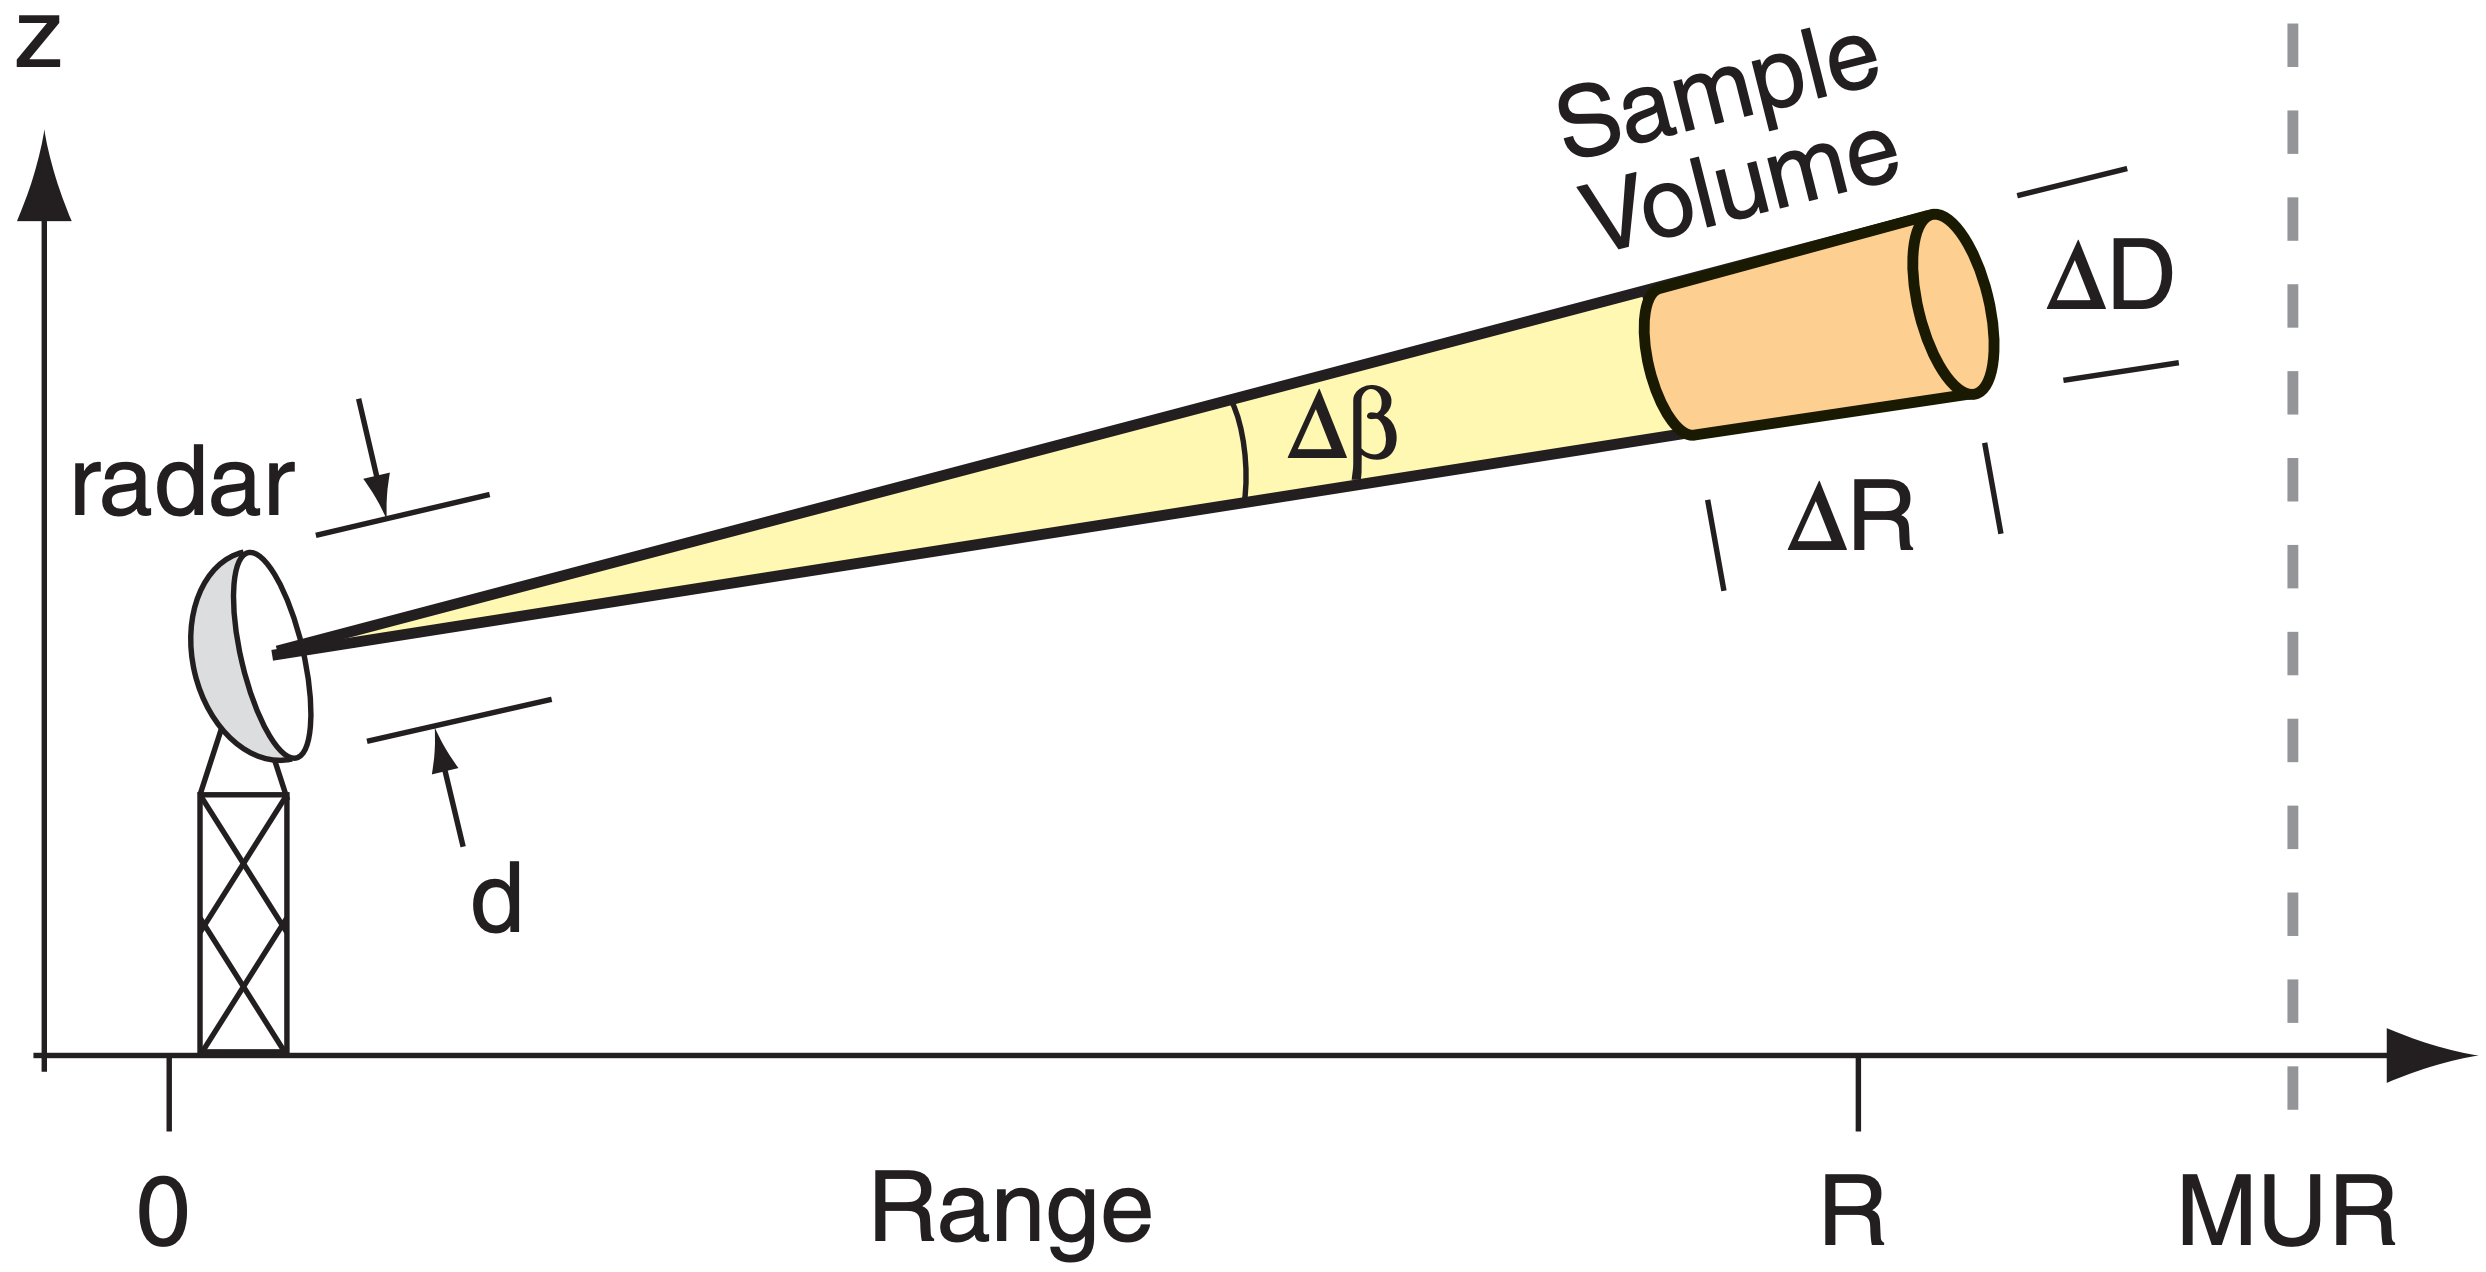
\includegraphics[width=1\linewidth]{Images/radar_concept.png}
    \vspace{1em}
    \caption{A typical meteorological radar - \cite{2022Weather}}
    \label{fig:radar}
\end{figure}
\newpage
% Các khái niệm cơ bản
\subsection{Basic terminologies}


\subsubsection{Weather Radar}
% \footnote{Tên tiếng Việt của các thuật ngữ sẽ được căn cứ dựa trên TCVN 12636-12 : 2021 \cite{vn_meteor_standard}}
% Radar thời tiết là một loại cảm biến có khả năng phát sóng vô tuyến (bước sóng trong phạm vi từ 250 - 1000 kW) \cite{2022Weather}. Để gia tăng cường độ sóng, một chảo antent (attenna dish) hình parabol được sử dụng nhằm hội tụ bước sóng. Radar có thể nâng và hạ (tuỳ theo yêu cầu) để thu nhập thông tin tại các vị trí chỉ định trong không gian 3 chiều.

Normally, weather radars are programmed to scan in an azimuth of $360^o$.
For every round, the radar will scan at a different altitude.
It usually takes about four to ten minutes for the radar to complete a full scan.

\begin{figure}[htp!]
    \centering
    \begin{subfigure}{\textwidth}
        \centering
        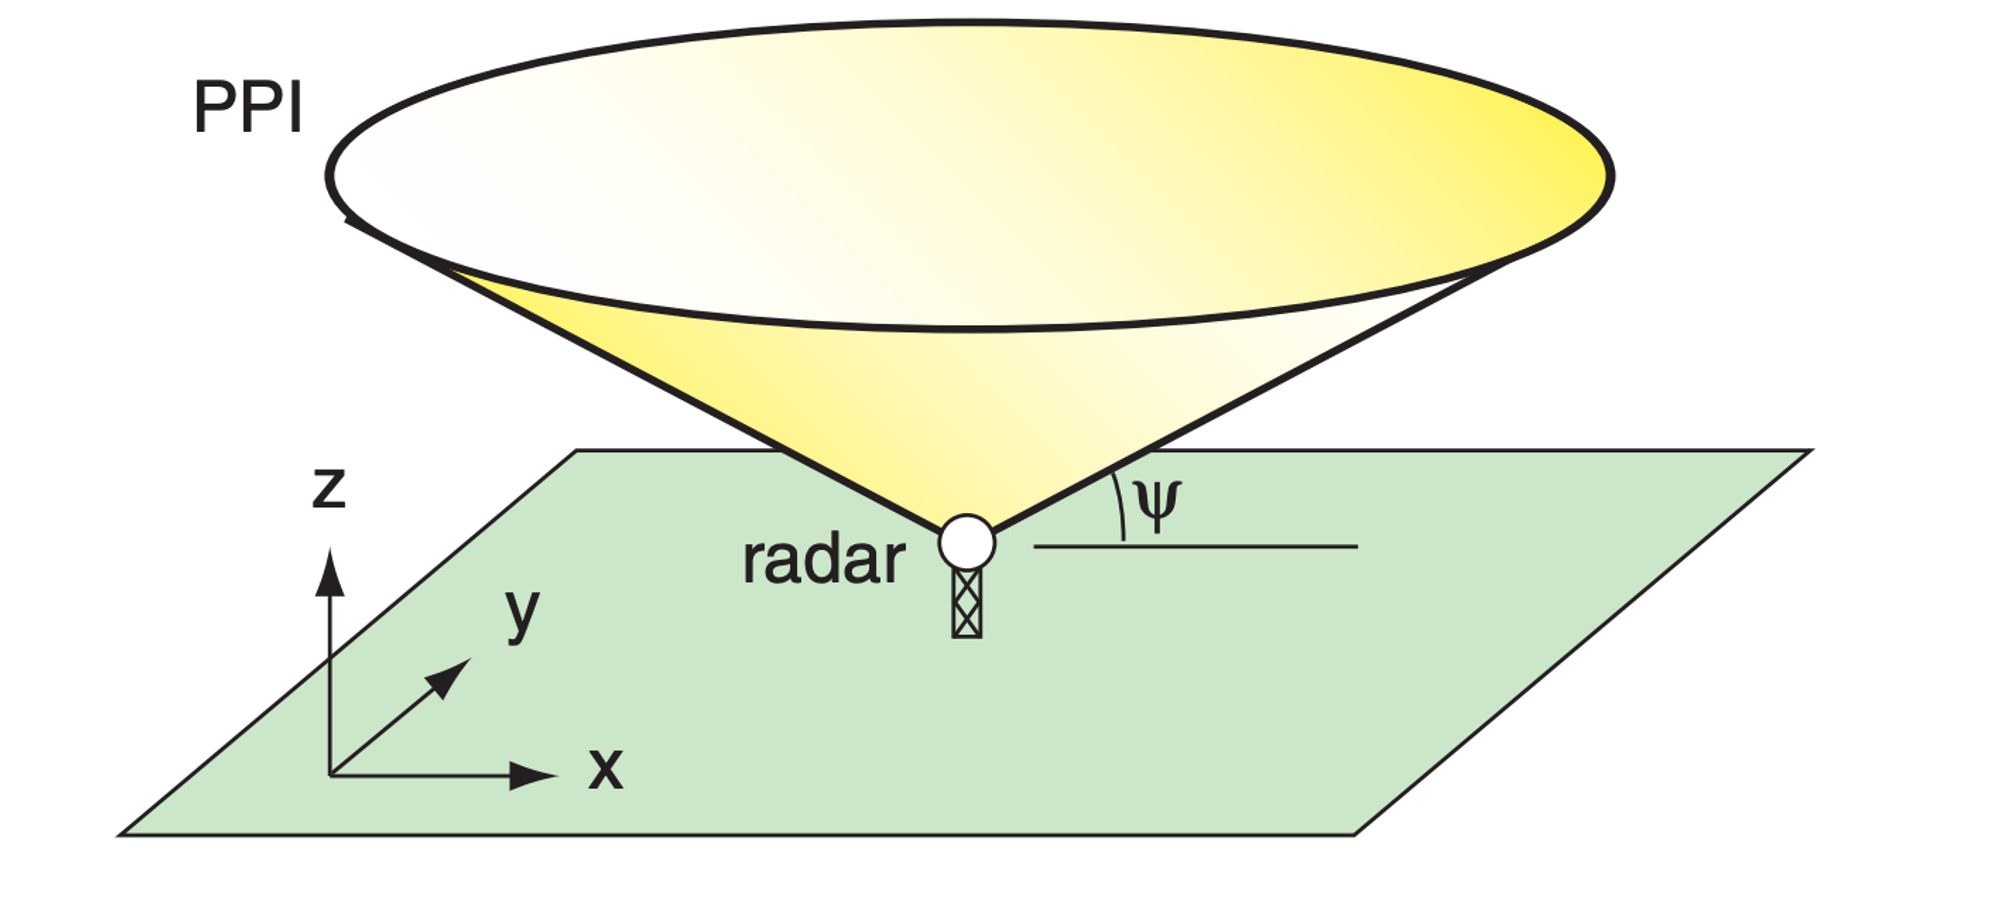
\includegraphics[width=0.85\textwidth]{Images/2.1-ppi.png}
        \caption{Plan-Position Indicator - PPI - \cite{2022Weather}}
        \label{fig:ppi}
    \end{subfigure}

    \begin{subfigure}{\textwidth}
        \centering
        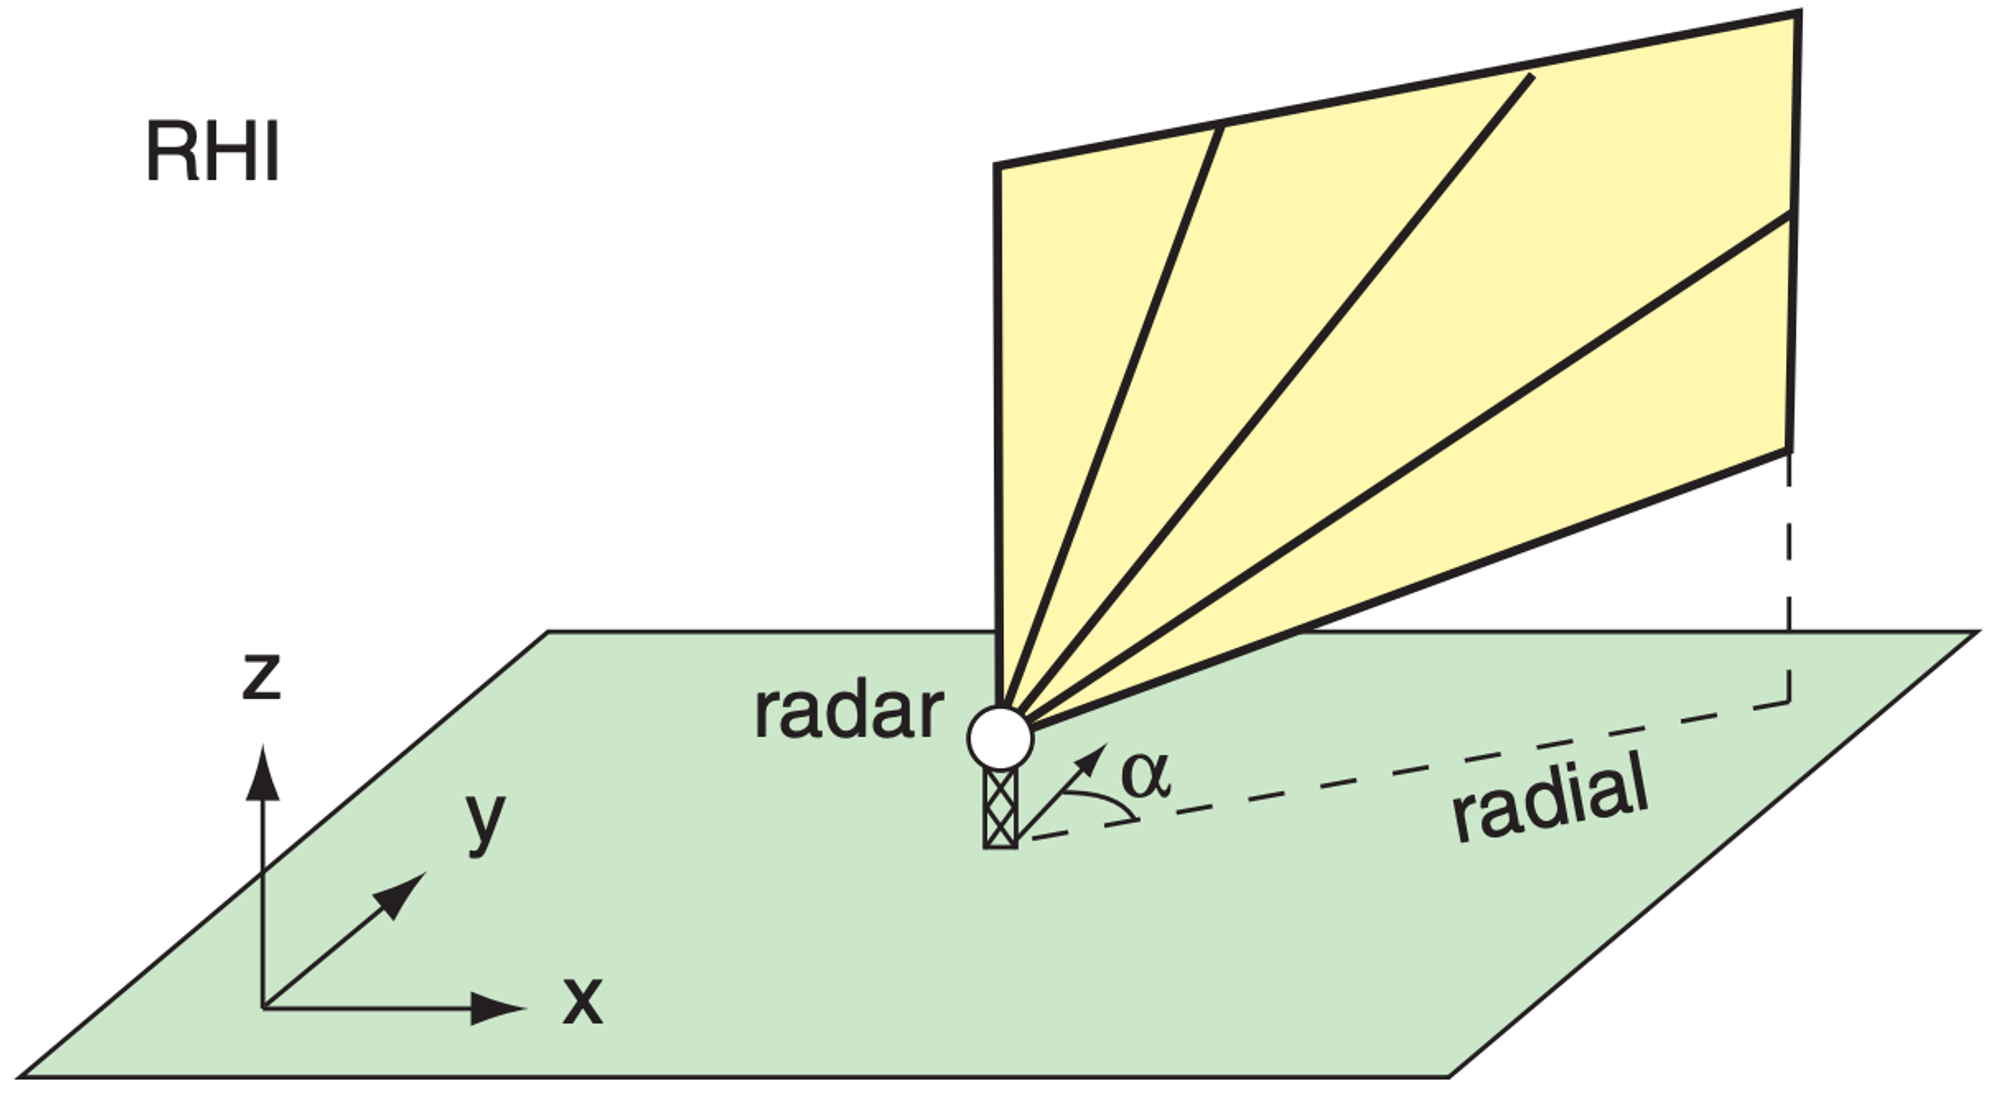
\includegraphics[width=0.85\textwidth]{Images/2.1-rhi.png}
        \caption{Range Height Indicator - \cite{2022Weather}}
        \label{fig:rhi}
    \end{subfigure}

\end{figure}

For PPI representation, the radar will scan the entire azimuth, but only at a certain altitude.
The final result would be similar to a map on a flat surface.

For RHI, in contrast, the radar retains the azimuth but increases in altitude.
The collected result gives viewers more details about the height and sizes of a meteorologist event.

\begin{figure}[H]
    \centering
    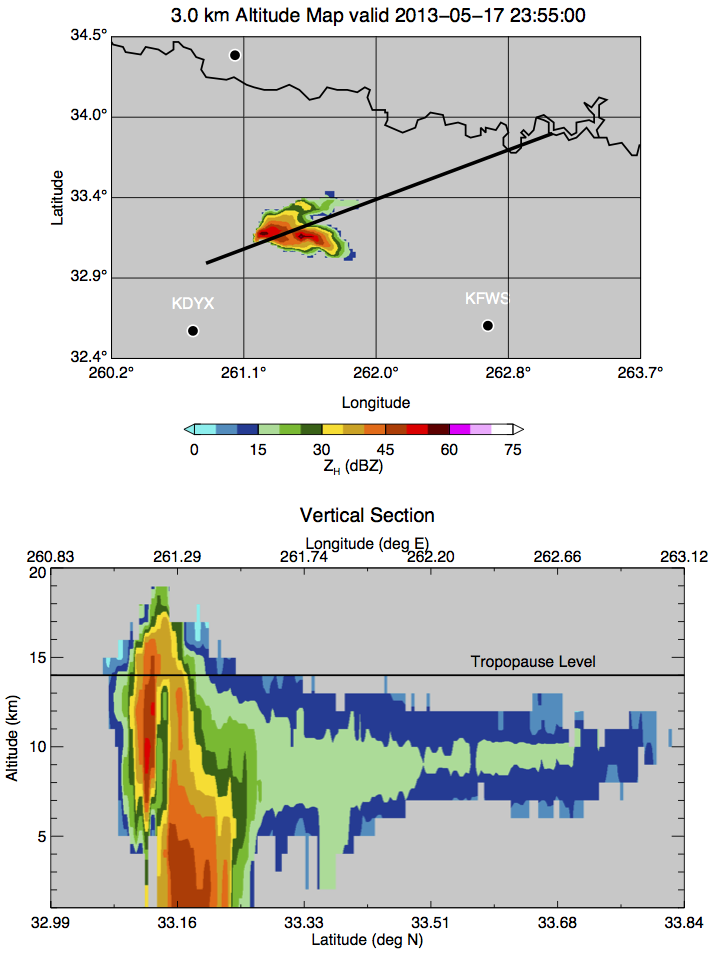
\includegraphics[width=\linewidth]{Images/2.1-ppi-and-rhi.png}
    \caption{Comparing the result between PPI and RHI - \cite{stackexchange-ppi-rhi}}
    \label{fig:ppi-and-rhi}
\end{figure}

\subsubsection{Radar equation and Reflectivity}
At a certain point in time, weather radar will emit a short pulse of radio wave ($\Delta t = 0.5 - 10 \mu s$).
Depending on the density of free molecules in the air (water vapor, smoke, ...), the energy of this wavelength will be partially absorbed.
The wavelength intensity that the radar receives will be less than the intensity of the original wave.
This ratio is expressed through \textbf{The radar equation} \cite{2022Weather}:

\[
    \left[ \frac{P_R}{P_T} \right]=\left[ b \right]\cdot\left[ \frac{|K|}{L_a} \right]^2\cdot\left[ \frac{R_1}{R} \right]^2\cdot\left[ \frac{Z}{Z_1} \right]
\]
\vspace{0.5cm}

Which, the variables of the equation include:
\begin{itemize}
    \item $|K|$ unitless:
          \begin{itemize}
              \item $|K|^2 \approx 0.93$ for droplets
              \item $|K|^2 \approx 0.208$ for ice crystal
          \end{itemize}
    \item $R (\text{km})$: distance from the radar to the target
    \item $R_1 = \sqrt{Z_1 \cdot c \cdot \Delta t / \lambda^2}$: ratio of distance
    \item $Z$: Radar's reflectivity
    \item $Z_1 = 1 \text{ mm}^6 \text{ m}^{-3}$: Radar's unit reflectivity
\end{itemize}

From the radar equation, we can derive the formula for reflectivity:
\vspace{0.5cm}
\[
    \text{dBZ} = 10\left[ \log\left( \frac{P_R}{P_T} \right) + 2 \log\left( \frac{R}{R_1} \right) - 2\log\left| \frac{K}{L_a} \right| - \log\left( b \right) \right]
\]
\vspace{0.5cm}

Meteorologists are usually interested in this number because it is proportional to the amount of precipitation.
\vspace{0.5cm}

\begin{table}[h]
    \centering
    \begin{tabular}{|c|c|}
        \hline
        Value (dBZ) & Weather               \\
        \hline
        -28         & Haze                  \\
        -12         & Clear air             \\
        25 - 30     & Dry snow / light rain \\
        40 - 50     & Heavy rain            \\
        75          & Giant hail            \\
        \hline
    \end{tabular}
    \vspace{1em}
    \caption{ Relation between reflectivity and precipitation - \citet{2022Weather}}
\end{table}

\begin{figure}[H]
    \centering
    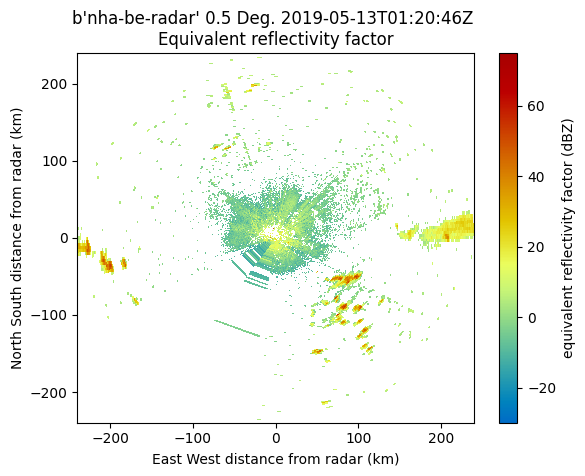
\includegraphics[width=0.75\textwidth]{Images/2.1-reflectivity_nhabe.png}
    \vspace{1em}
    \caption{Reflectivity from Nhà Bè radar}
    \label{fig:reflectivity-nhabe}
\end{figure}


\subsubsection{Radial velocity}

\begin{figure}[H]
    \centering
    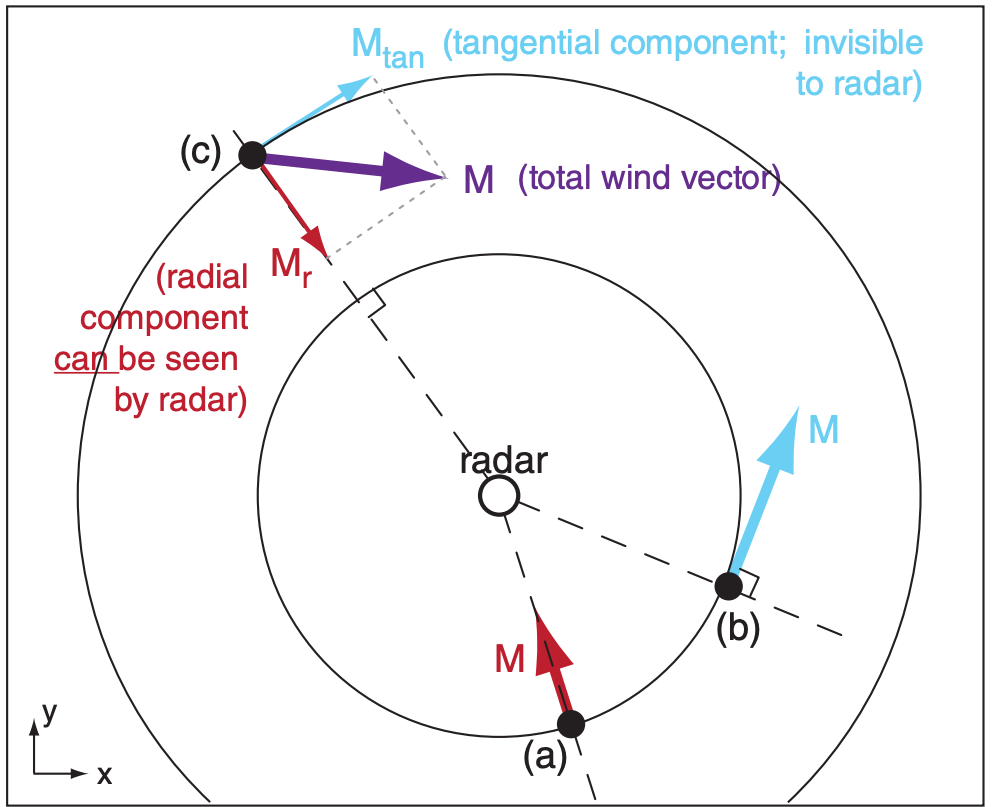
\includegraphics[width=.55\textwidth]{Images/2.1-radial-velocity.png}
    \vspace{2em}
    \caption{Illustrate the velocity situations that a Doppler radar can observe. (a) When the wind direction at point M coincides with the radius of the circle centered at the radar, the radar can determine the velocity at this point. (b) When the wind direction is tangent to the circle, the radar cannot determine the velocity. (c) Analyzing the wind direction at M into two perpendicular velocities, the radar can only determine the velocity vector along $M_r$.}
    \label{fig:radial-velocity}
\end{figure}

When the radio waves from these Doppler radars propagate to the molecules in the air, the displacement of these particles causes a phase shift between the transmitted and received signals. Radars rely on this information to calculate the wind velocity at various points in space.
\section{Common Data format in meteorology}
\subsection{SIGMET data format - raw format (Vaisala)}
\label{sigmet}
Vaisala is a Finnish company specializing in environmental and meteorological instrumentation. The RAW format (also referred to as SIGMET in some documents \cite{lrose_RadxConvert}) is one of the storage formats developed by the company to organize data output from their radar devices.

Some notable points about this format include:

\begin{itemize}
    \item The file content is divided into a \textbf{block}, each with a size of exactly 6144 bytes. This size aligns with the main storage size on older tape devices.
    \item The file typically consolidates data from all radar scanning sessions.
    \item Data records are organized within the scope of one block (6144 bytes). In the case of any remaining space in the block, it is padded with additional zeros.
\end{itemize}

With the aforementioned characteristics, the key advantages of the RAW format storage can be identified: \cite{raw_product_format_vaisala}

\begin{itemize}
    \item Compatibility with various tape types, which were commonly used devices in the past and are still widely used due to their cost-effective storage capacity.
    \item By storing data as blocks, SIGMET facilitates block-level error recovery in storage systems.
\end{itemize}

The main concern raised by the team is the mapping capability between the storage structure on the hard drive and the tape.

\subsection{NETCDF data format - Network Common Data Form}

NetCDF (Network Common Data Form) is a versatile file format designed explicitly for storing multidimensional scientific data. Within the netCDF library system, various binary formats are supported, each contributing to the flexibility and scalability of data management \cite{netcdf}. Notably, these formats include:

\begin{enumerate}
    \item Classic Format: Initially used in the first version of netCDF and remains the default choice for file creation.
    \item 64-bit Offset Format: Introduced since version 3.6.0, this format supports larger variable and file sizes.
    \item netCDF-4/HDF5 Format: Introduced in version 4.0, utilizing the HDF5 data format with some limitations.
    \item HDF4 SD Format: Primarily supports data reading.
    \item CDF5 Format: Synchronized support with the parallel-NetCDF project.
\end{enumerate}

All these formats exhibit self-description, with a detailed header part describing the file structure, including data arrays and file metadata in the form of attribute name/value pairs. This design ensures platform independence, with issues such as endianness being flexibly addressed through software libraries.

Consider a specific example of storing essential meteorological parameters such as temperature, humidity, pressure, wind speed, and direction in netCDF files. This illustrates the capability of this format in handling diverse scientific datasets, providing a powerful and flexible means to manage multidimensional information.

\begin{figure}[H]
    \centering
    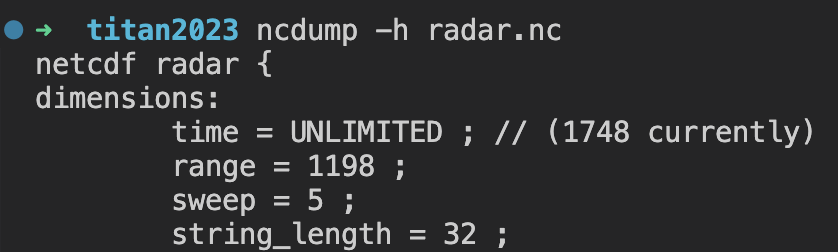
\includegraphics[width=1\linewidth]{Images/ncdump.png}
    \vspace{1em}
    \caption{Radar information in NETCDF format. The total dimensions of the dataset are 2975, grouped into 4 distinct labels.}
    \label{fig:enter-label}
\end{figure}

Starting from version 4.0, the netCDF API introduces the ability to use the HDF5 data format.
This crucial integration allows netCDF users to create HDF5 files, unlocking benefits such as significantly larger file sizes and support for unlimited dimensions.
This step marks a significant move towards leveraging the extended advantages of the HDF5 format.

NetCDF Classic and 64-bit Offset Formats are international standards of the Open Geospatial Consortium \cite{ogcnetcdf}, demonstrating the robustness and reliability in ensuring the compatibility and global scalability of the netCDF format.

\section{Related technologies}
\subsection{Apache Airflow™}

Apache Airflow™ stands as an open-source platform designed to manage data flow
within systems associated with data. In the face of the escalating challenge of
data pipeline management, Airflow emerges as a comprehensive solution,
automating and optimizing data-related workflows effectively \cite{airflow}.

Airflow not only aids in defining and managing the start and end times of each
data pipeline but also provides precise and detailed monitoring of the results
of each task. This becomes particularly crucial when ensuring the integrity and
reliability of the processed data.

With the ability to discern complex relationships between tasks through the
Directed Acyclic Graph (DAG) model, Airflow empowers administrators with tighter
control and flexibility in handling workflow processes. Its robust integration
with logging systems facilitates detailed activity tracking, assisting in issue
resolution and ensuring that every process aligns with expectations.

Simultaneously, the scheduling flexibility makes Airflow an excellent tool for
time and resource management. Its strong integration with various data sources
and extensibility through plugins allows Airflow to meet diverse needs in data
processing and task automation.

Apache Airflow not only delivers robust performance but also brings flexibility
and optimal technical features to data processing workflows. With its time
management capabilities, powerful logging integration, scheduling flexibility,
and scalability, Airflow stands as the top choice for enhancing performance and
control in data processing workflows.

\subsection{Kubernetes}

Kubernetes, an open-source system for managing and deploying highly flexible
applications in cloud and data center environments, has evolved into one of the
most widely adopted tools in the field of Information Technology \cite{k8s-doc}.
Originally developed by Google and later transferred to the Cloud Native
Computing Foundation (CNCF), Kubernetes aims to automate the deployment,
scaling, and management of containerized applications, alleviating the burden on
developers and system administrators. The platform offers a unified foundation
for deploying, scaling, and managing containerized applications across multiple
servers.

Kubernetes operates based on key concepts such as Pods, Services, ReplicaSets,
and various other abstractions, creating a flexible environment for application
deployment and management. This fosters an environment where developers can
easily build applications, and system administrators can efficiently maintain
them.

Beyond supporting traditional deployment models, Kubernetes paves the way for
innovative strategies like Continuous Deployment (CD) and Microservices. With
the ability to automate many aspects of the development and deployment process,
Kubernetes plays a crucial role in constructing and sustaining complex,
flexible, and scalable systems.

\subsubsection{Kubernetes Components}

Introducing essential concepts for managing and deploying applications,
Kubernetes provides an effective and flexible environment. The main components
of Kubernetes include Pod, ReplicaSet, Deployment, and Service.

\begin{figure}[H]
    \centering
    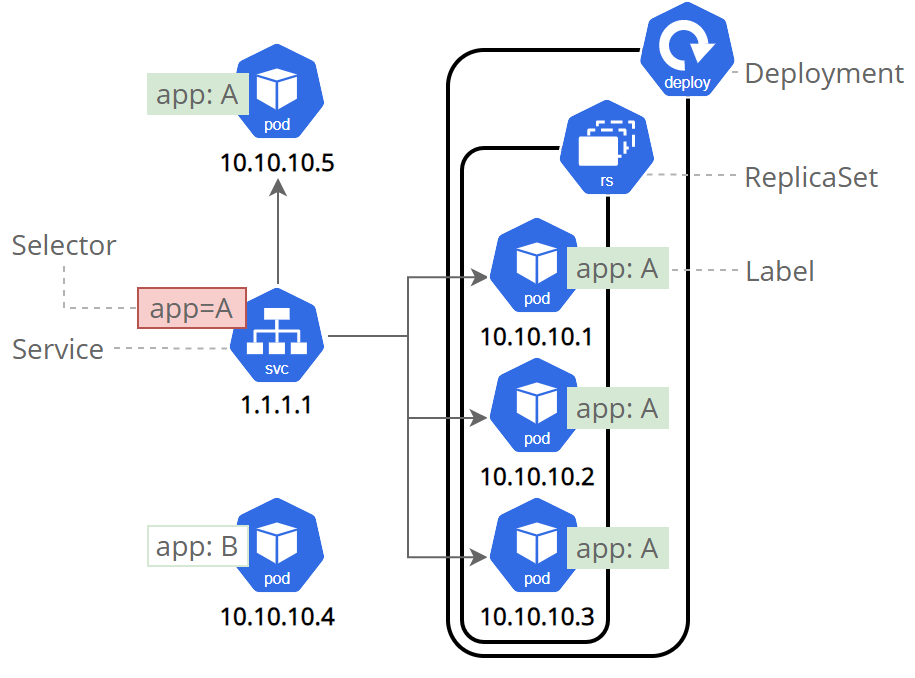
\includegraphics[width=0.75\linewidth]{Images/3.4-k8s-comps.png}
    \caption{Overview of Kubernetes Components - Kubernetes}
    \label{fig:k8s-comps}
\end{figure}

In Kubernetes, a \textbf{Pod} serves as the fundamental unit, representing a
collection of containers that share a common workspace. Within the same Pod,
containers collaborate by sharing network and storage resources, fostering
interaction and enabling the construction of intricate applications.

The \textbf{ReplicaSet}, a crucial resource in Kubernetes, ensures a designated
number of Pods operate in a specified manner. In the event of a Pod failure or
shutdown, the ReplicaSet automatically initiates the creation of a new Pod to
replace it. This mechanism ensures the application's stable state by
guaranteeing a defined number of Pods are consistently operational.

For managing the deployment and updating processes of applications,
\textbf{Deployment} is a key component in Kubernetes. It articulates the desired
state of the application and orchestrates the updating of the ReplicaSet to
achieve that state. Deployment provides versatile management capabilities,
facilitating the deployment of new versions, rollbacks, and updates without
disrupting the service.

The \textbf{Service} resource in Kubernetes furnishes an HTTP port to Pods,
generating a unique IP address and DNS name for a cluster of Pods. This enables
seamless communication among applications within the cluster and with external
environments. Service effectively simplifies the intricacies of handling
multiple Pods and IP addresses, offering a straightforward means of accessing
services within the Kubernetes environment.

Typically, large-scale systems leverage Kubernetes in their software development
and deployment processes. This adoption brings several advantages, including
efficient resource management and self-recovery capabilities. Kubernetes
optimizes resource utilization, ensuring optimal performance and reducing waste.
Additionally, it automatically addresses issues during operations, enhancing
high availability.

However, the technology is not without its challenges, including a steep
learning curve for beginners. Mastery of diverse knowledge areas such as
computer networking and containerization is necessary. Moreover, deploying and
maintaining Kubernetes demands significant resources, both in terms of personnel
and hardware, particularly for smaller organizations.

\subsubsection{High Availability in Kubernetes}

High Availability is a crucial factor in the success of any system. In
Kubernetes, High Availability is achieved through the combination of several
features, including self-healing, load balancing, and auto-scaling.

First, Kubernetes uses \textbf{Deployment}, a type of \textbf{Controller} for
managing replicas. Through Deployment, we can easily perform horizontal scaling,
which is the process of increasing the number of replicas of a Pod. This
mechanism ensures that the application can handle numerous requests without
compromising performance. Moreover, in case of a Pod failure, a Deployment makes
sure that a new Pod is created to replace it, ensuring the amounts of predefined
replicas is always maintained.

At network layers, Kubernetes uses \textbf{Service} for communication between
various components within or outside the cluster. Instead of directly accessing
Pods, other components can access Services, which will redirect the request to
the appropriate Pod. When Pods are replaced, the Service will automatically
update the routing rules to ensure the request is sent to the correct Pod.
Outside the cluster, Kubernetes also uses \textbf{Ingress} to manage external
access to Services. Instead of specifying the direct node IP address, Clients
can abstract it by using only the URL or hostname.

Finally, at the storage level, Kubernetes provides Persistent Volumes. By doing
so, applications can be agnostic to the underlying storage infrastructure. This
allows for easier management and scaling of storage resources. Not only that,
depending on the provided \textbf{Storage Class}, Kubernetes makes sure that the
data is replicated to multiple nodes, ensuring data availability in case of node
failure.

To summarize, Kubernetes provides a robust set of features to ensure High
Availability. By leveraging these features, we can build a highly available
system that can scale with our load, while also being resilient to failures.

\subsection{LROSE}

LROSE (Lidar Radar Open Software Environment) is a project supported by the
National Science Foundation (NSF) with the goal of developing common software
for the Lidar, Radar, and Profiler community. The project operates based on the
principles of collaboration and open source. The core software package of LROSE
is a collaborative effort between Colorado State University (CSU) and the Earth
Observing Laboratory (EOL) at the National Center for Atmospheric Research
(NCAR) \cite{lrose}.

Originating from the need for a unified software environment for processing
Lidar and Radar data in atmospheric science research \cite{lrose}, the project
addresses complexities related to integrating data from various observation
platforms, including Lidar, Radar, and Profiler. These components are designed
to meet the specific needs of meteorologists and researchers working with remote
sensor data.

LROSE is widely used in meteorological research, including studies related to
cloud and precipitation processes, boundary layer dynamics, and other
meteorological phenomena. The software supports the analysis of observation data
collected from ground-based tools such as Lidar and Radar. LROSE seamlessly
integrates with a variety of model and atmospheric analysis tools to optimize
its capabilities. Researchers often integrate LROSE into numerical weather
prediction models as well as other data assimilation techniques, creating a
flexible and powerful system.

\begin{figure}[H]
    \centering
    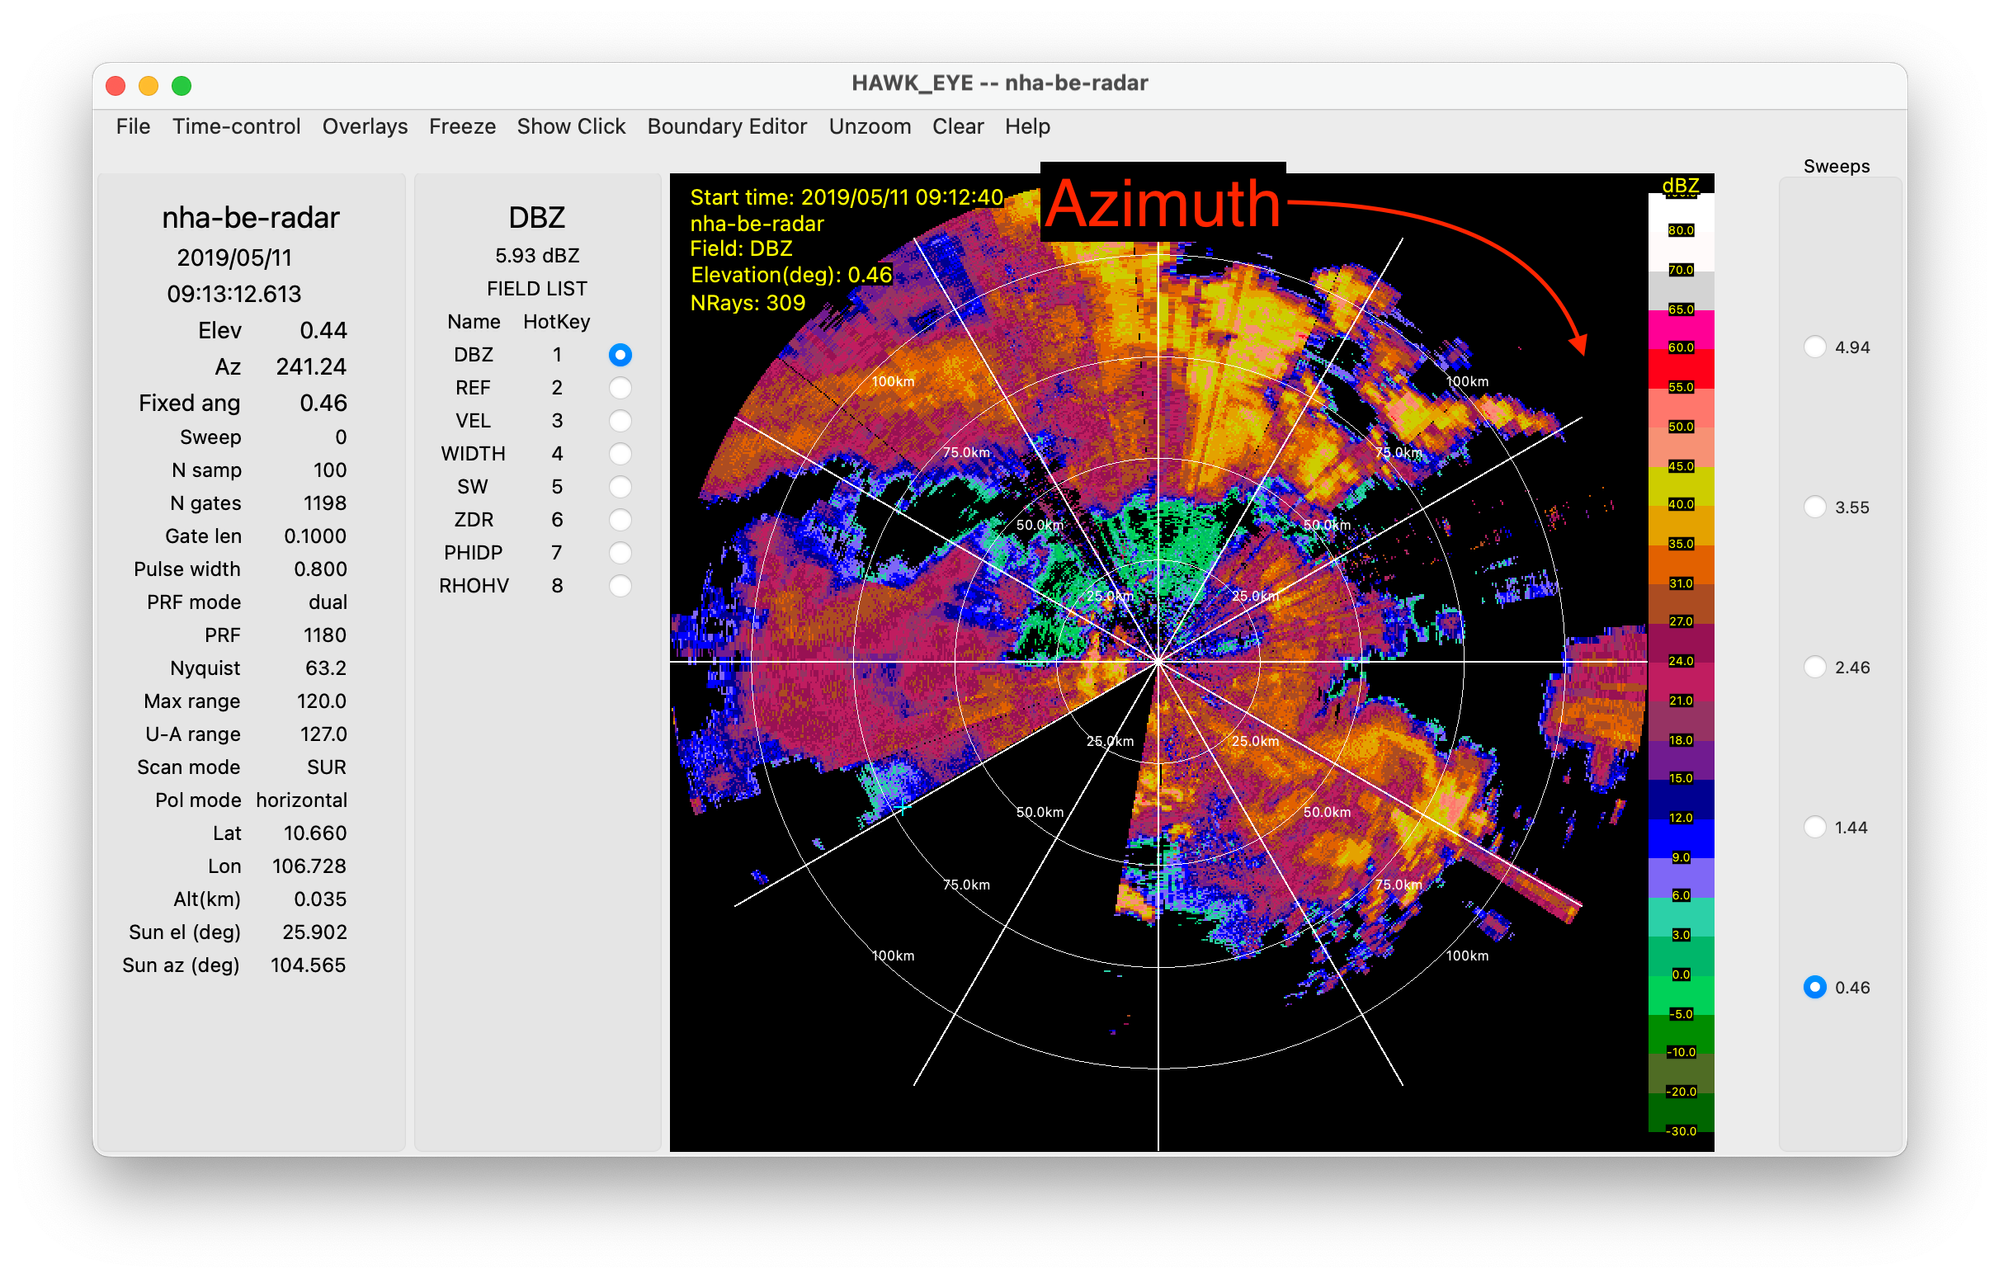
\includegraphics[width=0.8\linewidth]{Images/3.5-hawk-eye.png}
    \caption{Hawk Eye, Lidar and Radar visualization tool of LROSE}
    \label{fig:hawk-eye}
\end{figure}

The project actively encourages participation from a large scientific community,
promoting the exchange of ideas, algorithms, and improvements for the software.
Regular updates and contributions from users contribute to the continuous
development and refinement of LROSE.

\subsection{FastAPI}
FastAPI is a high-performance web development framework based on Python,
distinguished by its unique and advanced technical features designed to address
challenges in building high-performance and flexible APIs.

It is one of the rare frameworks that fully leverages type hints and
async/await. Type hints help clearly define the data types of variables and
functions, making the source code more explicit and understandable.
Additionally, support for async/await enables handling multiple requests
concurrently without slowing down the processing, especially crucial for
applications requiring high responsiveness and scalability.

With robust support for type hints, FastAPI automatically generates API
documentation based on Python's data types. This not only helps reduce errors in
the source code but also generates automatic API documentation, streamlining the
development process and interaction with the API. FastAPI also supports industry
standards such as OpenAPI and Swagger, providing a flexible way to manage
resources, authentication, and user accounts.

Beyond its technical prowess, FastAPI excels in concurrent handling and
performance. The special support from asyncio allows FastAPI to process multiple
requests simultaneously without impeding processing speed. This capability
ensures smooth and fast-running applications while facilitating scalability, a
crucial factor for large research projects with evolving requirements over time.

FastAPI not only simplifies the development process but is also designed with
the goal of optimizing the development experience. It lays the foundation for
easily building production-ready APIs thanks to its integrated best practices.
With this combination, FastAPI is not just a powerful tool but also an efficient
and flexible solution for projects that demand reliability and scalability in
the future.

\newpage
\chapter{System Analysis and Design}
\input{Chapters/3.0-Overview.tex}
\section{Exploratory Data Analysis}



\section{Data Model}
\input{Chapters/3.2-data_model.tex}
\section{System Architecture}
\begin{figure}[H]
    \centering
    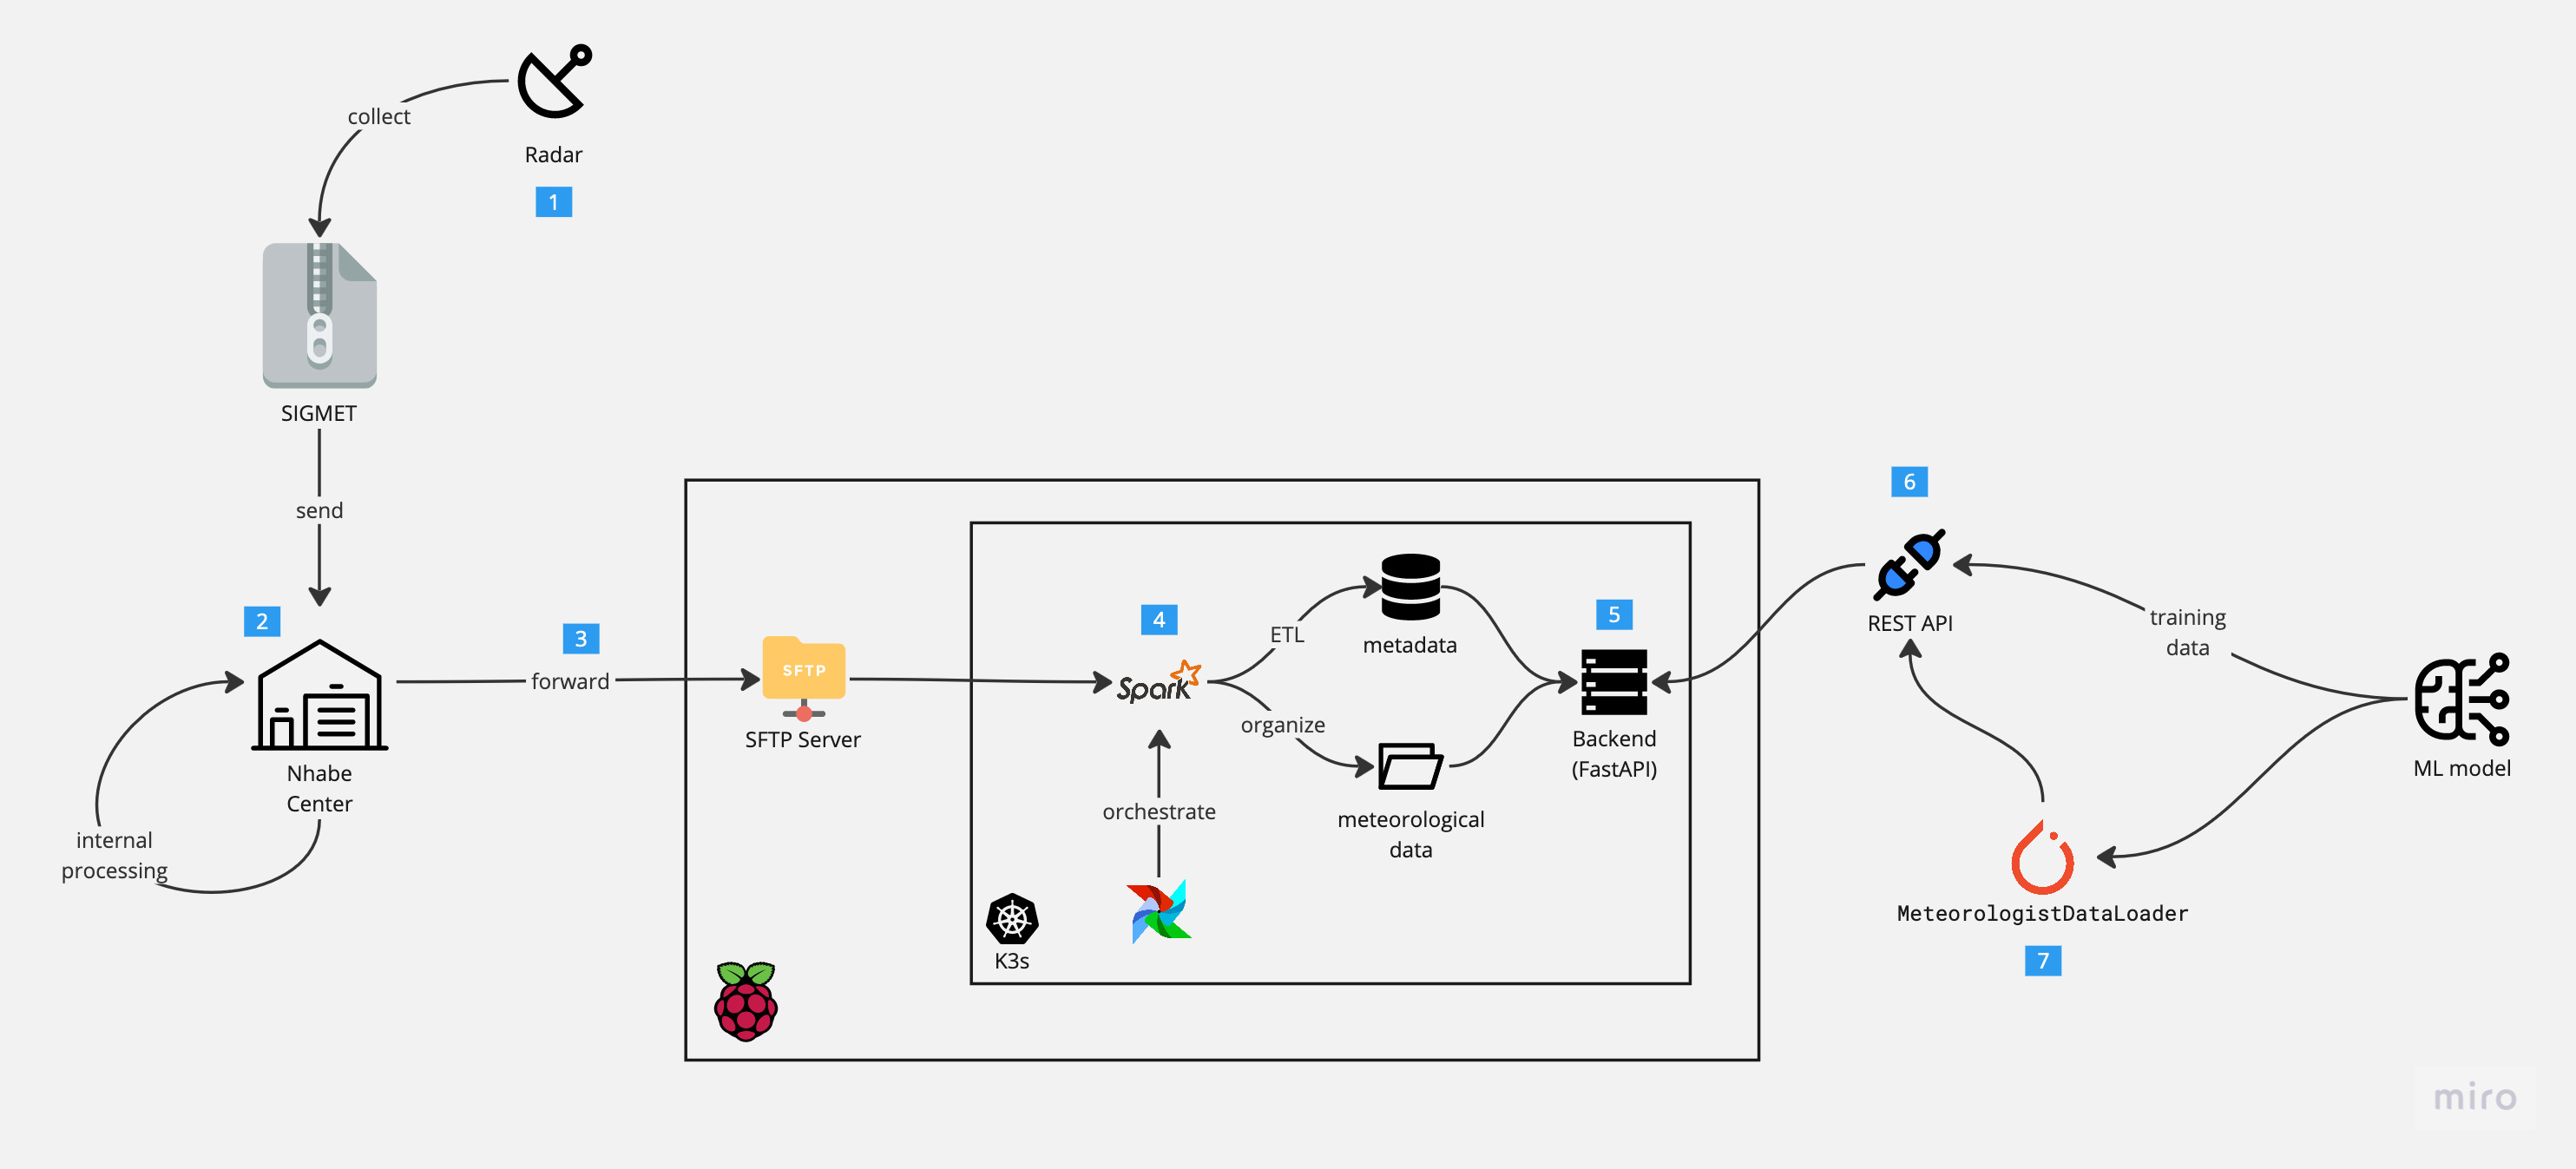
\includegraphics[width=\linewidth]{Images/4.1-architecture.jpg}
    \vspace{1em}
    \caption{System Design - Proposed}
    \label{fig:sow}
\end{figure}
\vspace{0.5cm}
Based on the requirements set by stakeholders and after studying the existing system, the team proposes the design and implementation of a system titled "Integrated Database for Short-Term Prediction in Hydrometeorology." Figure \ref{fig:sow} illustrates the team's design template.
\newpage
\section{Current System}
The design comprises seven main sections. Among them, the part of the system currently operational at the Nha Be observation station is depicted in the first two steps:

Firstly, in step 1, during each specific cycle, a geostationary satellite collects meteorological data. Some received indices include:
\begin{enumerate}
    \item Doppler Spectrum Width
    \item Mean Doppler Velocity
    \item Reflectivity
\end{enumerate}

All this information is transmitted to the Nha Be observation station in the SIGMET format \ref{sigmet}. Subsequently, in step 2, the meteorological staff at the Nha Be station records and processes the transmitted data according to their operational requirements.


\newpage
\chapter{Implementation}
\section{Data Processing}
The implementation phase of the team will be an extension to the current system,
which is outlined in Figure \ref{fig:sow}.

In step 3, the team will set up a simple SFTP server. SFTP is a straightforward
and widely used protocol, supported by numerous libraries and tools for
communication based on this protocol. Additionally, compared to FTP, the
mentioned protocol ensures security during data transfer. Depending on the
permissions, the team may assist the observation station in constructing scripts
to automatically forward processed files or allow manual file submission.

Once files are uploaded to the SFTP server, the team utilizes Airflow to
orchestrate all existing ETL workflows in the overall system. Currently, the
team pauses with a single DAG to process data from the Nha Be observation
station. Airflow monitors newly added files on our SFTP server and initiates the
ETL process. The choice of Apache Spark is based on the volume and complexity of
the data. If the data size per new SIGMET file is manageable with Python alone,
without the need for Spark, it will not be employed in this step.

Meteorological data, upon reaching the team's infrastructure, will be bifurcated
into two main streams: Metadata, such as creation date, size, timestamp, etc.,
will be stored in a traditional Relational Database Management System (RDBMS).
Specifically, PostgreSQL is chosen due to its popularity and the team's
familiarity. Storing metadata here facilitates rapid query responses without
direct access to the raw data. Common queries may include:

\begin{itemize}
    \item What timestamps are being recorded? (e.g., from 21/11/2023 to
    17/12/2023)
    \item At timestamp $x$, what are the geographical coordinates of the radar?
    \item What fields of data are currently stored?
\end{itemize}

Additionally, the database acts as an index, quickly identifying the storage
location of raw data.

For specific hydrometeorological data, the team finds it inefficient to store
them directly in conventional DBMS. Simultaneously, storing data in files still
maintains a reasonable overall size. Therefore, the team decides to separate the
raw data and store it directly in files. This approach, combined with the
previously mentioned indexes, accelerates the retrieval process.

To facilitate data queries for models, machine learning, AI, etc., the team will
develop a simple backend server using Python's FastAPI at step 5. In step 6, the
backend receives query data in REST API format, queries the metadata DB and data
files, and returns the achieved results. During different training instances,
Machine Learning entities can connect to this server to retrieve data.

It's worth mentioning that the entire system will be developed and operated in a
containerized manner and will be deployed on the Kubernetes platform. This
reflects the system's ability to maintain high availability and ease of solution
maintenance. In this illustration, the team will deploy it on a cluster of
Raspberry Pi-embedded computers.

Lastly, in step 7, the team proposes an additional consideration. If suitable,
the team may build a DataLoader to swiftly serve other model-making groups.
Considering the popularity of Pytorch in AI, the team will initially approach
this platform.

\section{Endpoint architecture}

\subsection{Programming languages and Libraries}

C\# was selected for this project because of its widespread popularity in
enterprise applications and its capability to operate across various operating
systems following the release of .NET Core. This feature significantly enhances
deployment flexibility, allowing the application to be utilized in diverse
environments. 

Additionally, we have incorporated ASP.NET Core specifically version 8 into our
technology stack. By leveraging ASP.NET Core, we benefit from a robust,
well-supported framework that facilitates the development of scalable and secure
web applications. It seamlessly integrates with C\#, enabling us to utilize a
consistent programming environment while also exploiting features such as
dependency injection, a vast ecosystem of middleware, and a strong configuration
system that is suited to modern web applications.

ASP.NET Core 8 brings forward improvements in areas such as minimized startup
times, reduced memory footprint, and enhanced security features, making it an
ideal choice for developing scalable and secure web applications. The choice
also underscores our commitment to developing applications that are both
efficient and future-proof, ensuring that they perform optimally on both Windows
and non-Windows platforms. This alignment with .NET Core’s cross-platform
capabilities ensures that our project remains versatile and adaptable to the
evolving technological landscape.

Optionally, we have integrated the Nuxt framework into our technology stack.
Nuxt is a progressive Vue framework that is used for building more robust and
versatile web applications. It simplifies the development process by handling
various aspects of the web infrastructure, such as server-side rendering, static
site generation, and automatic code splitting. This inclusion enriches our
application's interactivity and user experience, providing a seamless and
dynamic interface for users.

\subsection{Command Query Responsibility Segregation}

The Command Query Responsibility Segregation (CQRS) is an architectural pattern
that distinctively separates the tasks of reading data (queries) and writing
data (commands) within a software application. This separation splits
responsibilities into two main components:

\begin{itemize}
\item \textbf{Command Side}: This component manages operations that modify the
system's state. It handles incoming commands from clients or external systems,
conducts validations, and updates the data store accordingly. This side is
essential for maintaining the integrity and accuracy of data modifications
within the application.
\item \textbf{Query Side}: Dedicated to data retrieval, this component processes
all read requests. It fetches data from the appropriate sources, ensuring that
the information provided is accurate and reflects the current state of the data
store.
\end{itemize}

Key advantages of employing the CQRS pattern are:

\begin{itemize}
\item \textbf{Scalability}: CQRS allows for the independent scaling of the read
and write components based on their respective workloads, which can
significantly enhance system performance.
\item \textbf{Flexibility}: With the separation of concerns, different storage
and optimization strategies can be applied to the reading and writing processes.
This flexibility enables the use of the most appropriate tools for each
function, optimizing efficiency.
\item \textbf{Event-Driven Architecture Compatibility}: The use of CQRS often
complements event-driven architectures, where changes in the system's state are
captured and managed as events. This compatibility ensures that the architecture
is dynamic and responsive to changes in business requirements.
\end{itemize}

\subsection{Project Structure}


\section{Datastore}
\subsection{The purpose of storing data directly as raw file}
In the comprehensive compilation acquired during the recent field excursion, an
array of invaluable data was meticulously gathered, meticulously chronicled, and
thoughtfully analyzed. Specifically, our focus gravitated towards the
operational activities conducted within the radar center situated in the Nha Be
district. Operating at the pinnacle of technological advancement, the radar
center diligently executes periodic scans of the atmospheric conditions,
facilitating the meticulous documentation and exportation of a SIGMET file,
which serves as a repository encapsulating a myriad of meteorological phenomena
and atmospheric dynamics.

The SIGMET file, serving as the quintessential embodiment of scientific rigor
and methodological precision, meticulously records a plethora of critical
parameters and meteorological variables. Among the salient features meticulously
delineated within this archival masterpiece are the discerning metrics of
reflectivity and wind radial velocity. Reflectivity, a fundamental metric in
radar meteorology, is an indispensable parameter delineating the intensity of
electromagnetic waves returned to the radar antenna from various atmospheric
particles, thereby furnishing crucial insights into the spatial distribution and
intensity of precipitation within the monitored region. Furthermore, the wind
radial velocity, an elemental component in meteorological analysis, delineates
the rate and direction of atmospheric motion along the radial axis relative to
the radar antenna. These metrics serve as a vital tool in elucidating the
intricate dynamics of atmospheric circulation, enabling meteorologists to
decipher prevailing wind patterns, identify regions of convective activity, and
forecast the trajectory of severe weather phenomena with enhanced accuracy and
precision.

Yet, amidst the effervescent tapestry of meteorological data acquisition and
analysis, a conundrum of paramount importance arises: the optimization of data
storage and retrieval mechanisms. It is within this crucible of inquiry that the
proposition to store meteorological results directly within the file repository
assumes a mantle of significance, heralding a paradigm shift in data management
practices.

Indeed, the inherent multidimensionality of meteorological data, encapsulated
within its tripartite tensor structure, underscores the imperative for a
streamlined approach to data storage and retrieval. By eschewing aggregation and
denormalization techniques, we advocate for a direct integration of results
within the archival framework, thereby fortifying the foundations of data
integrity and computational efficiency.

Moreover, the proposition to leverage the existing ETL (Extract, Transform,
Load) system developed by Vaisala, as utilized by our esteemed National Center
for Hydrometeorological Forecasting, emerges as a beacon of pragmatism and
resourcefulness. In a landscape fraught with technological complexities and
budgetary constraints, the utilization of pre-existing infrastructure represents
a judicious allocation of resources, affording seamless integration and
interoperability across disparate data management platforms.

In summation, the decision to store meteorological data directly within the file
repository, without resorting to further aggregation techniques, emerges as a
testament to both pragmatism and foresight. By embracing this approach, we not
only enhance the accessibility and usability of meteorological datasets but also
lay the groundwork for a new era of scientific inquiry and meteorological
prognostication, fortified by the pillars of technological innovation and
methodological rigor.


\subsection{Extracting data from each of the radar center}
We have authored a script, albeit not yet integrated into the operational
system, designed to facilitate the redirection of the SIGMET (Significant
Meteorological Information) file from the data center to our preconfigured
Storage Server.

Presently, the script is implemented in Python to ensure platform-agnosticism.
Accompanied by a concise setup script, it will be poised for execution on the
radar center's machinery.

MinIO has been employed as an unstructured data repository owing to its
compatibility with the S3 (Simple Storage Service) protocol. As the system
matures in the distant future, transitioning to AWS S3 should be
straightforward. The underlying logic and API for interfacing with the storage
infrastructure remain largely invariant during such a migration.

\begin{lstlisting}[language=Python, caption={Part of the script for uploading data to Storage}]
file_path = pathlib.Path(args.filename)

s3_client = boto3.client(
    "s3",
    endpoint_url=os.getenv("S3_HOSTNAME"),
    aws_access_key_id=os.getenv("S3_ACCESS_KEY_ID"),
    aws_secret_access_key=os.getenv("S3_SECRET_ACCESS_KEY"),
)
_ = s3_client.upload_file(file_path, os.getenv("S3_BUCKET"), generate_new_name(file_path.name))
\end{lstlisting}

At present, we adhere to a specific nomenclature for data file naming:
\texttt{<year><month><day>T<hour><minute><second>}. This naming convention
confers the advantage of expedited data retrieval for a particular time of day.
Leveraging S3 Prefix filtering facilitates the selection of multiple data points
within a given time frame, ranging from a second to potentially a year.

For instance, to query data for a specific day (e.g., 2024-03-15), utilizing the
UNIX path wildcard, we can express our query as:

\begin{lstlisting}[language=sh]
ls 20240315T*
\end{lstlisting}

\newpage

Analogously, the same query can be executed using the \texttt{boto3} library in
Python:

\begin{lstlisting}[language=Python, caption={Querying data in 2024-03-15}]
def query_with_wildcard(bucket_name):
    s3_client = boto3.client('s3')
    
    response = s3_client.list_objects_v2(
        Bucket='nha-be-radar',
        Prefix='20240315T'
    )
        
    return [obj['Key'] for obj in response['Contents']]
\end{lstlisting}

Moreover, although our naming convention deviates somewhat from the ISO-8601
standard for timestamp representation, the inclusion of the letter \textbf{T}
aids in swiftly identifying datetime components within the naming structure.

One limitation of this naming convention is its inability to support wildcard
querying for a central time component. Consider the scenario necessitating data
retrieval for a specific hour daily. Utilizing the UNIX wildcard, this can be
depicted as:

\begin{lstlisting}[language=sh][H]
ls 202403*T09*
\end{lstlisting}

The utilization of an internal wildcard here implies the absence of an efficient
mechanism for querying such objects presently. The current recourse involves
maximal prefixing (e.g., \texttt{Prefix=202403}), followed by subsequent
filtering in Python.

\subsection{Data Explorer}
Besides S3-compatible API for accessing the storage, our solution also provides some alternative ways
for preview the data storage. This can be used for manual intervention (in case of failure), or simply for
the radar center's operators to preview.

First, there is an online explorer that can be access from the web browser. As
you can see from Figure \ref{fig:minio-home}, the web UI is very user-friendly
and easy-to-use. With the use of IAM (shorts for Identity and Access Management)
and \textbf{Policies}, the admin user of our entire system can restrict what a
tenant (or a radar center) can see and what should be hidden.

\begin{figure}[H]
    \centering
    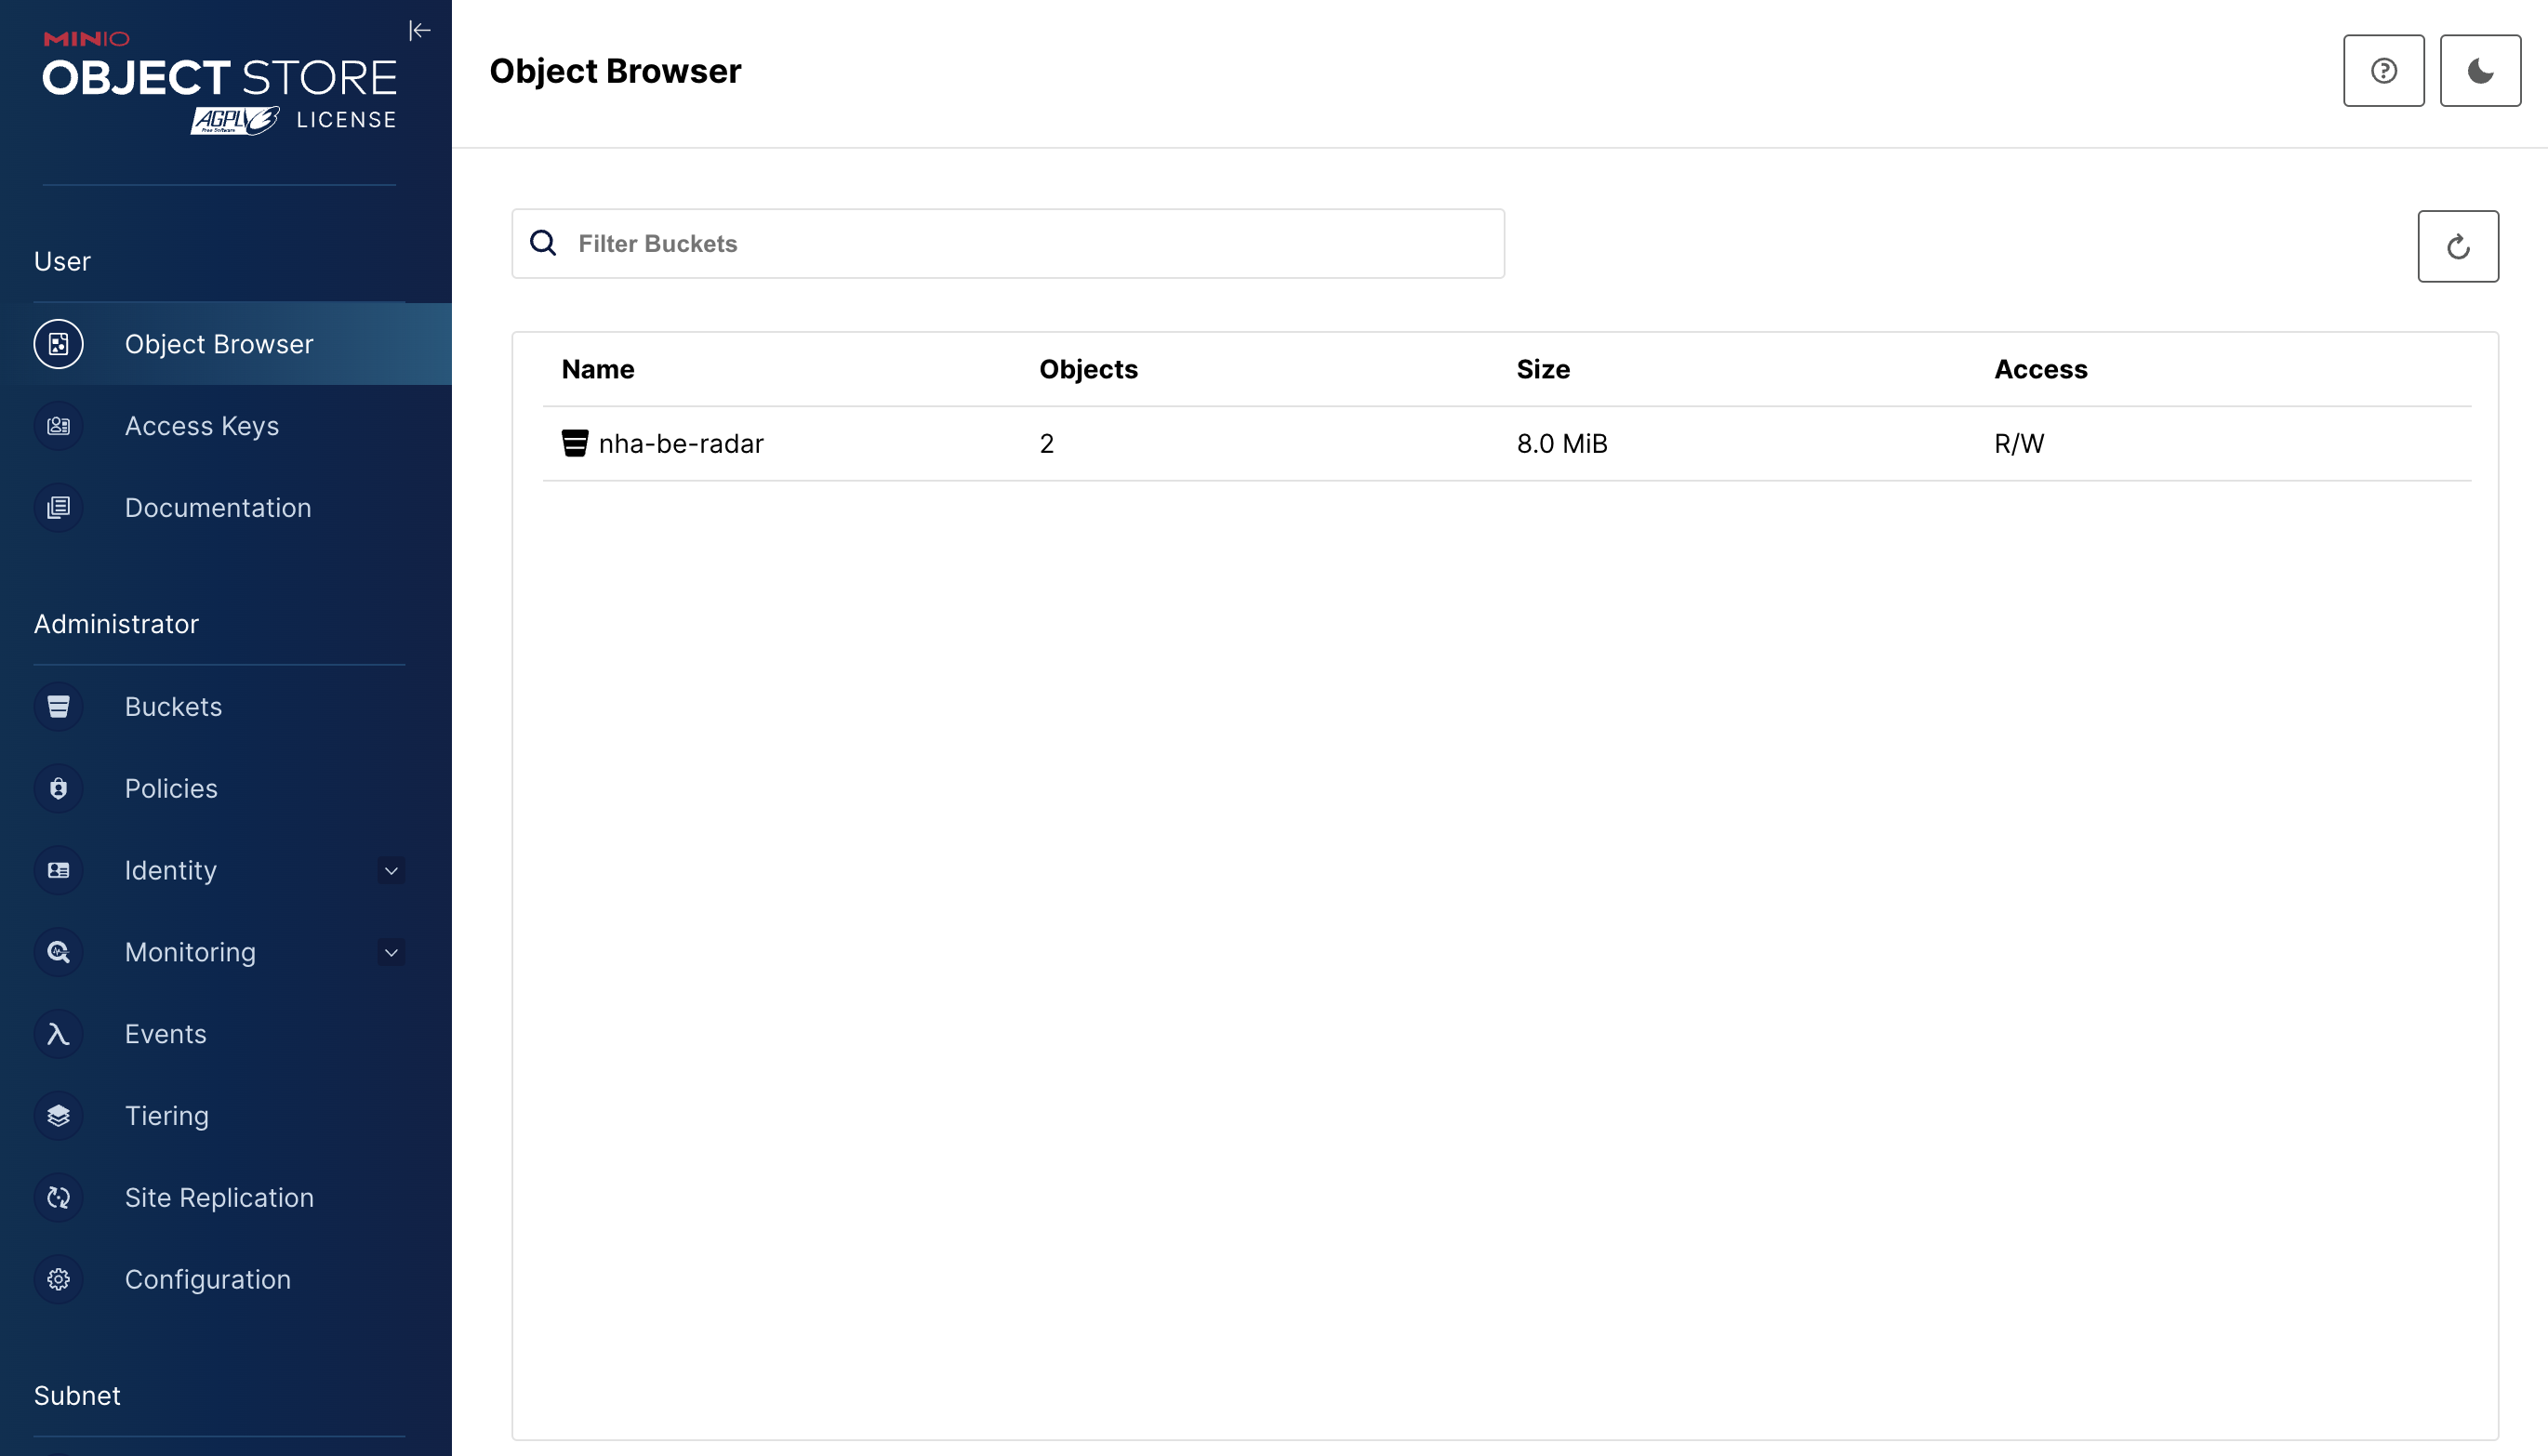
\includegraphics[width=0.8\linewidth]{Images/4.3-datastore/minio-bucket.png}
    \vspace{1em}
    \caption{MinIO web interface provides a clear and intuitive way to explore the storage}
    \label{fig:minio-home}
\end{figure}

Currently, as of the time of writing, our system has been self-hosted on a small
Raspberry Pi server. The explorer has been set up with necessary load balancing,
DNS and SSL/TLS registering correctly. Anyone can visit
\url{https://explorer.meteor-flow.com/} to see the server running. Figure
\ref{fig:minio-files} shows some of the files that our team has prepared beforehand.

\begin{figure}[H]
    \centering
    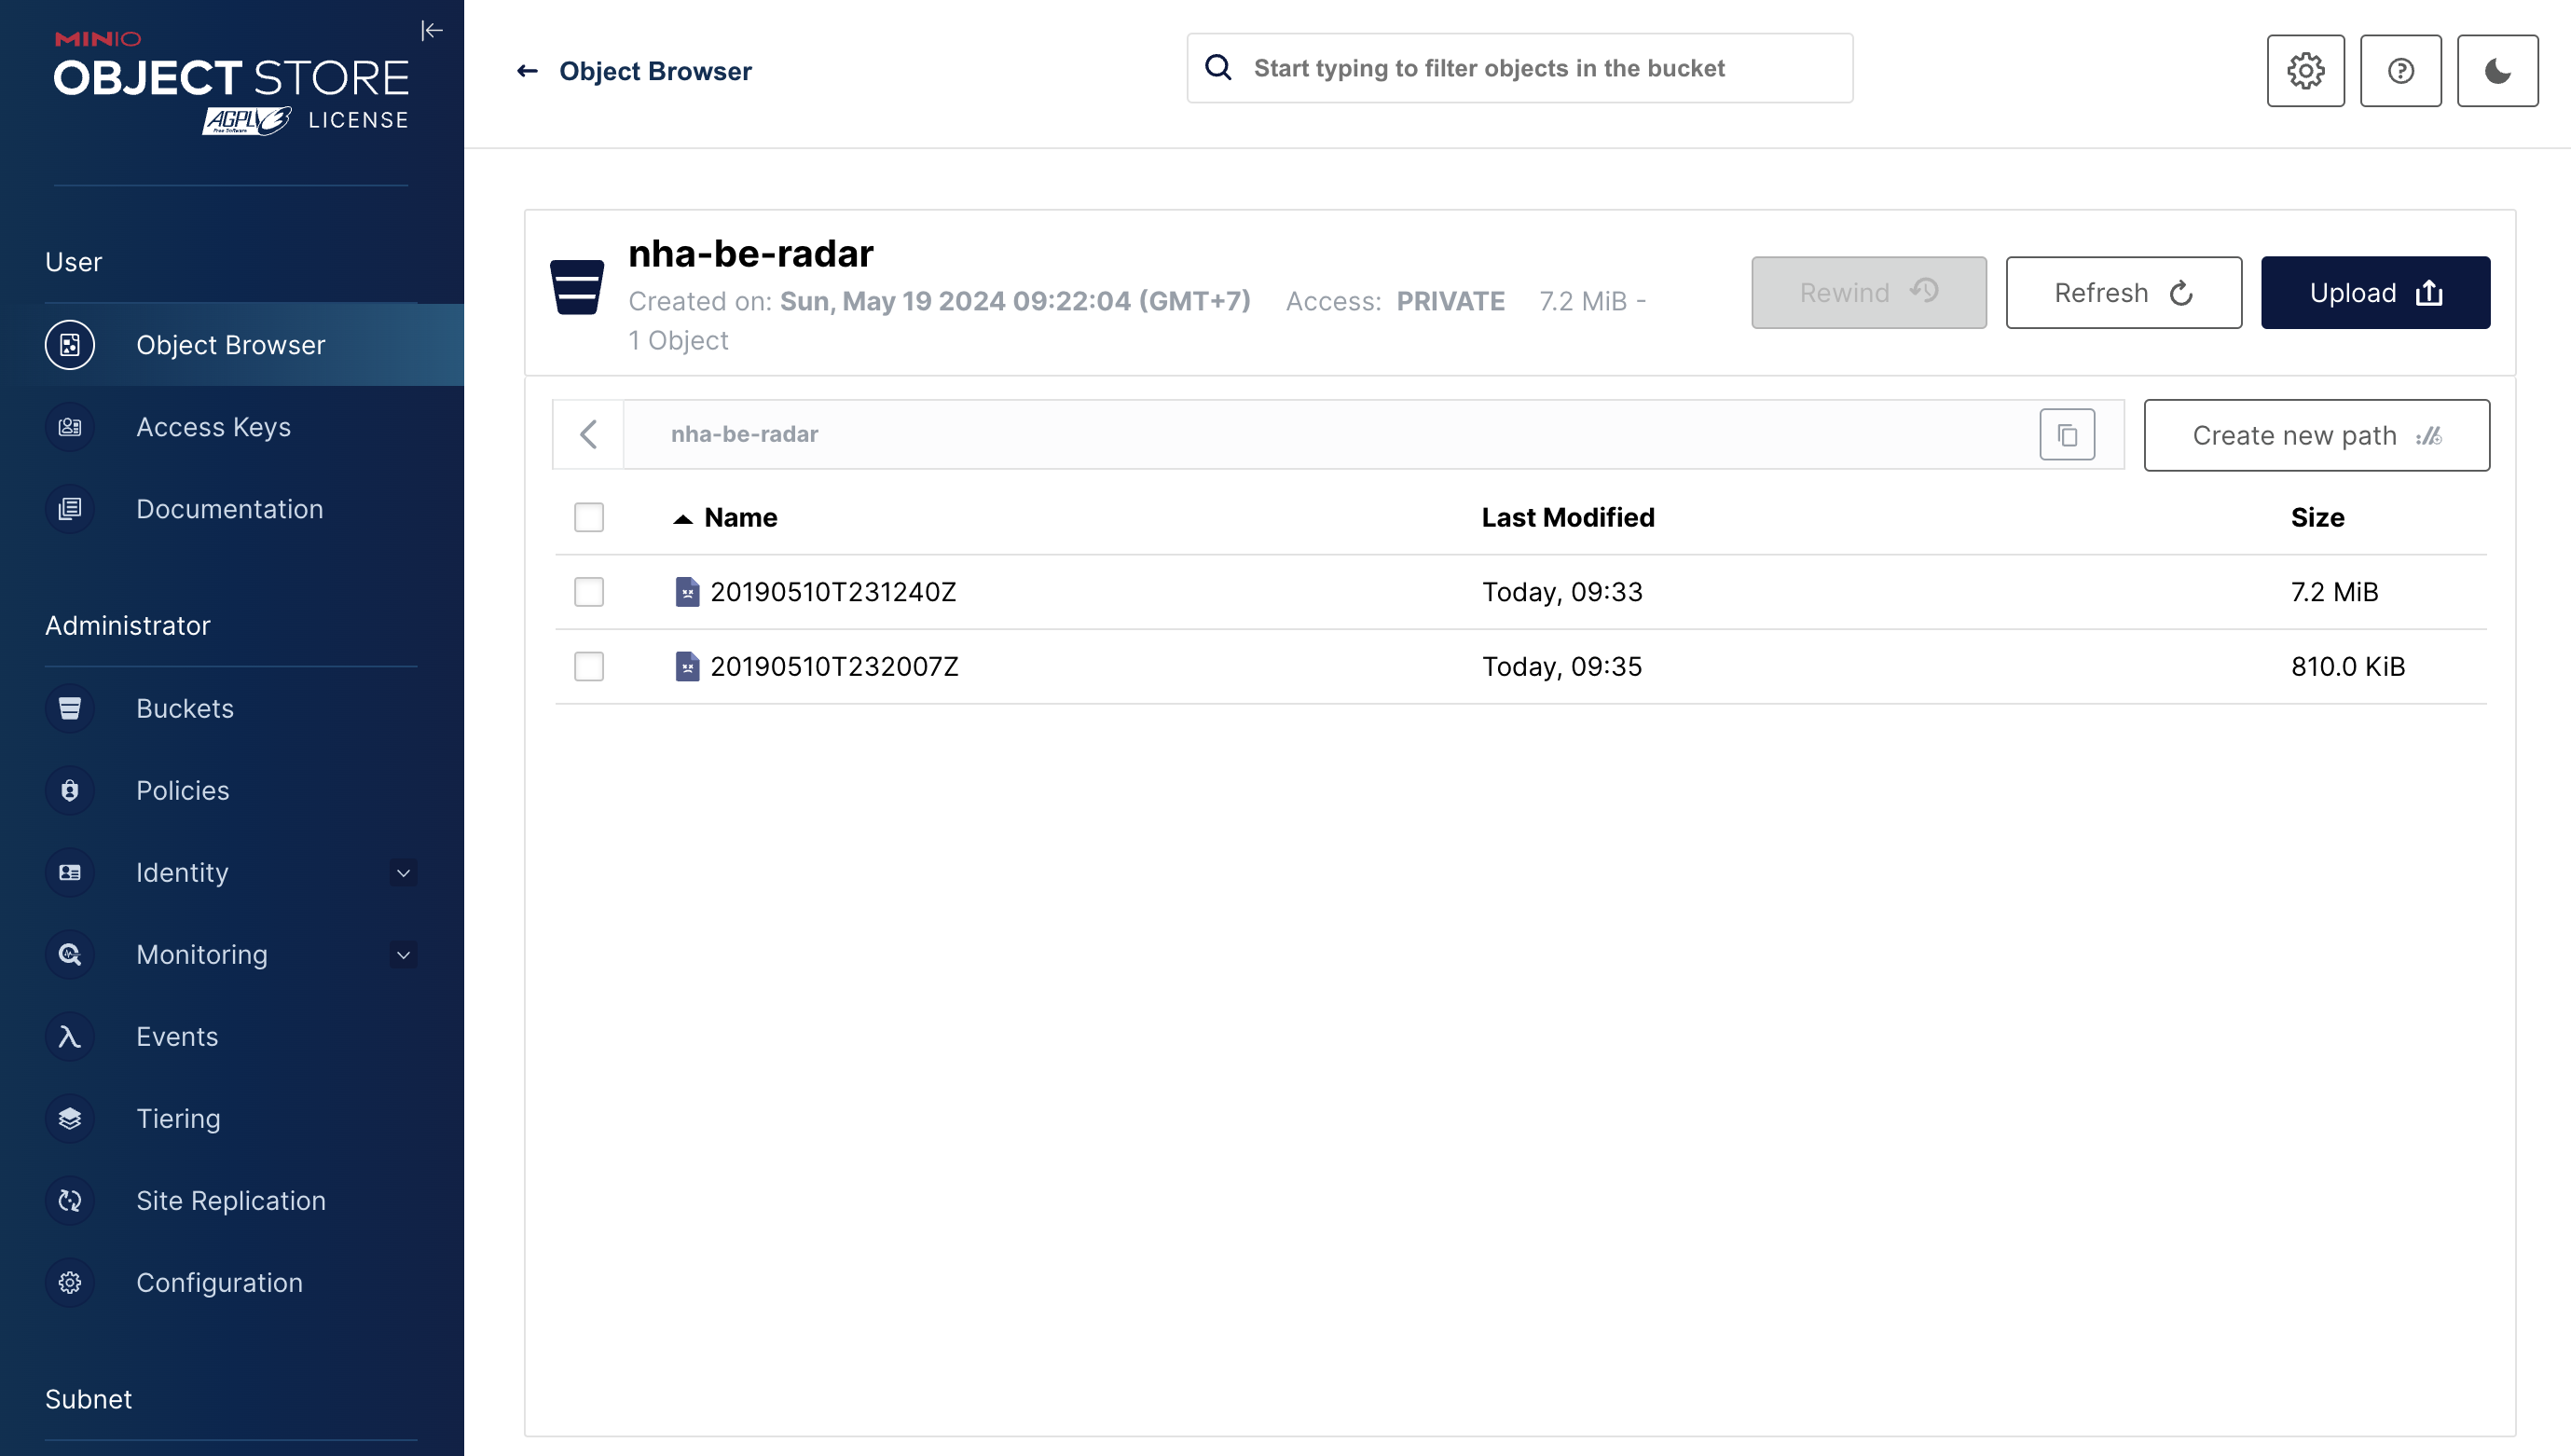
\includegraphics[width=0.8\linewidth]{Images/4.3-datastore/minio-files.png}
    \vspace{1em}
    \caption{Some radar files are currently being stored on the storage}
    \label{fig:minio-files}
\end{figure}


Not stopping at that, our system can also work with any other S3-compatible
client. One notable example of this is Cyberduck. In the future, our team can
research for more compatible protocols, such as FTP or SFTP.

\begin{figure}[H]
    \centering
    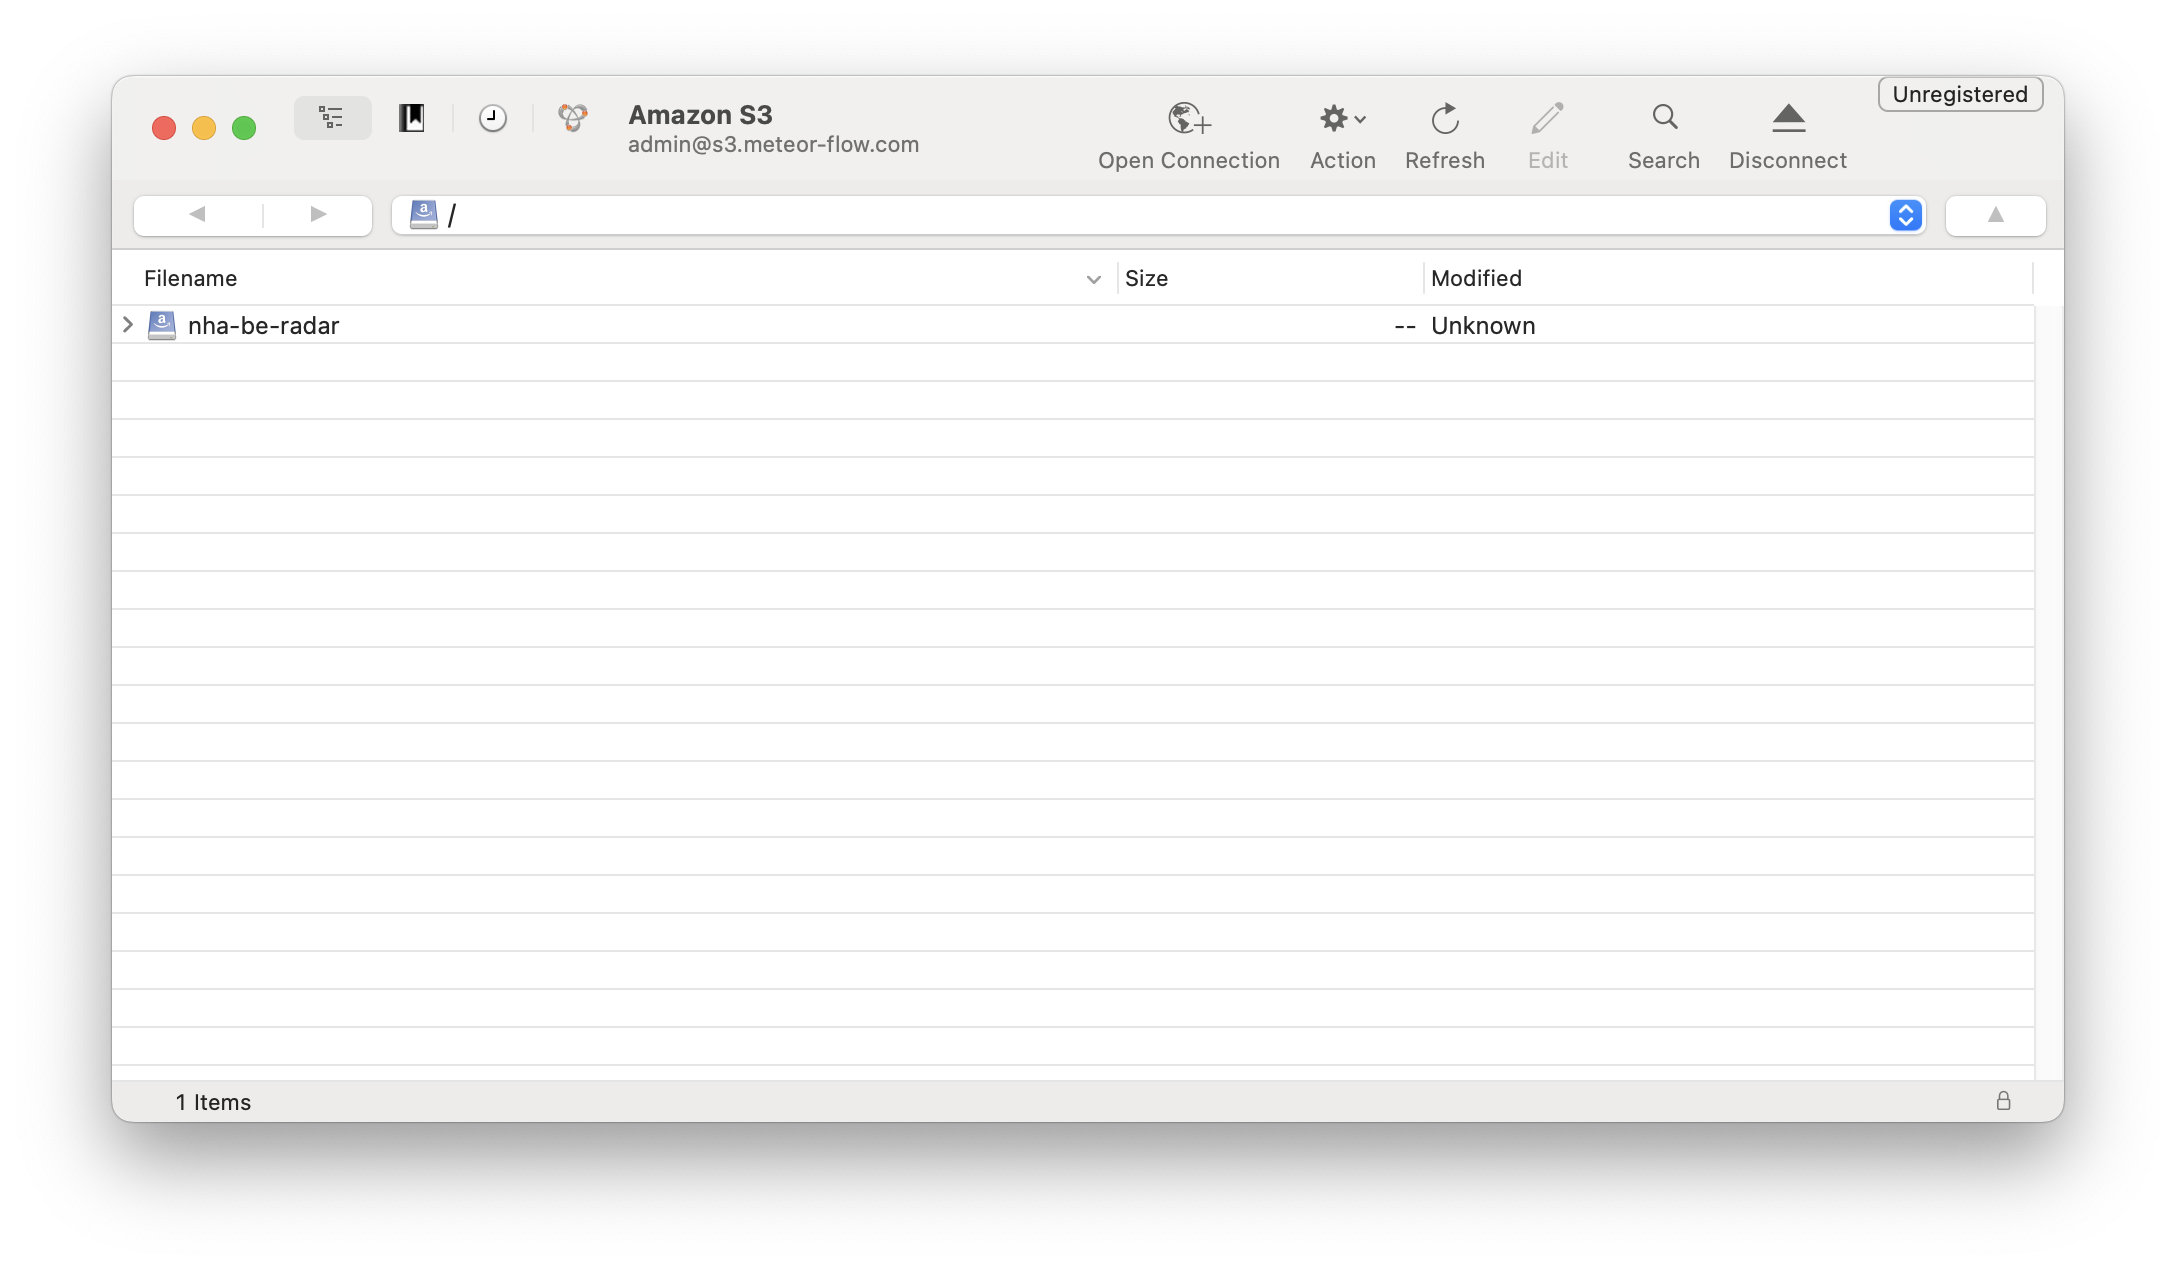
\includegraphics[width=0.6\linewidth]{Images/4.3-datastore/s3-client.png}
    \vspace{1em}
    \caption{Using Cyberduck to view data on the platform}
    \label{fig:s3-client}
\end{figure}



\chapter{Testing and Validation}
\section{Unit Test}
\input{Chapters/5.1-unit_test.tex}
\section{Integration Test}
During the Integration Test phases, our team makes sure that not only does our system run correctly at every part,
but also that the system as a whole works as expected. To do that, we first start with a Test Plan.

\subsection{MeteorFlow Test Plan}

\begin{center}
    \begin{tabular}[H]{|r|r|}
        \hline
        Project Name & MeteorFlow \\
        \hline
        Created Date & TBD        \\
        \hline
        Release Date & TBD        \\
        \hline
    \end{tabular}
\end{center}


\begin{tabular}[H]{|r|r|r|r|}
    \hline
    Component              & Start Time & Assignee               & Notes \\
    \hline
    ETL files and REST API & TBD        & Thuy Nguyen, Kiet Tran & Notes \\
    \hline
\end{tabular}


\subsection{MeteorFlow Test Report}

Release Date: TBD


\newpage
\chapter{Future enhancement}
\section*{Improve into a Weather Data Platform (WDP)}
The Weather Data Platform (WDP) is developed to become a comprehensive solution for harnessing the power of weather data. The system is designed to meet the specific requirements of meteorologists, scholars, academic researchers, and developers from various fields, including freelancers, businesses, and Non-governmental Organizations (NGOs). WDP serves as a centralized hub for integrating weather data, analysis, and various features.

With the desire to evolve into a Weather Data Platform, we aim for the perfection and diversification of weather information. Not just a data table but a comprehensive experience. In the future, in addition to continuing to build the proposed integrated database, we promise to further research to expand and develop this integrated database into a weather data platform with the following development directions:
\begin{enumerate}
    %\item Use Software Development Life Cycle (SDLC) methods like Agile to efficiently develop and deliver the product.
    %\item Differentiate between core and extended features.
    %\item Decide whether the product should be fixed or expandable.
    %\item Monitor and adopt new technologies in the weather and forecasting field to improve data quality and predictions.
    \item \textbf{Non-linear Data:} Expand beyond basic data integration, focusing on providing non-linear, detailed, and multi-source data to help users explore more about the surrounding environment.
    \item \textbf{Artificial Intelligence Understanding:} Use artificial intelligence to understand the language of weather, from minor changes to major events, creating a deep and intelligent weather information source.
    \item \textbf{Interactive User Interface:} Not just accessing information but also interacting with weather forecasts. The user interface will be where users express curiosity and interact directly with the data.
    \item \textbf{Geospatial Information Connection:} Leverage geographical information systems to provide a contextualized, localized view of weather forecasts. This helps users understand the impact of weather on their surroundings.
          %\item Build an integrated weather data, analysis, and other data sources platform.
    \item \textbf{Performance Optimization:} Ensure quick and consistent responsiveness under all conditions.
    \item \textbf{Data Security:} Enhance data security to ensure the security and integrity of weather information.
    \item \textbf{Advanced Forecasting System:} Research and integrate artificial intelligence to improve forecasting capabilities and provide accurate forecast information.
    \item \textbf{Testing and Optimization:} Conduct system testing to ensure stability and address any potential issues. Optimize performance if necessary.
    \item \textbf{Deployment and Maintenance:} Deploy the system and maintain a regular update cycle to ensure that it consistently delivers accurate and reliable weather information.
\end{enumerate}

\newpage
\chapter{Conclusion}
In this study, we have successfully built a Proof-of-Concept with high applicability, aiming to streamline the steps in the conventional workflow.
This is a crucial step towards optimizing and enhancing operational efficiency in both research and practical contexts.

Our goal was to create a flexible system with high adaptability, helping to simplify complex steps in the workflow.
In doing so, we not only contribute to increasing efficiency but also alleviate the workload pressure on personnel, creating favorable conditions for creativity and focus on core tasks.

We didn't just stop at developing the system but also proposed flexible deployment strategies, emphasizing easy integration into the current working environment of those involved in information gathering and weather forecasting tasks.



\bibliographystyle{plainnat}
\bibliography{refs}

\end{document}